\documentclass[11pt, oneside]{article}
\usepackage{geometry}
\geometry{letterpaper}
\usepackage[parfill]{parskip}    % Activate to begin paragraphs with an empty line rather than an indent
\usepackage{graphicx, amssymb, amsthm, amsmath, ragged2e, algorithm}

\usepackage[noend]{algpseudocode}
\usepackage{scrextend}
\newtheorem{theorem}{Theorem}
\newtheorem{lemma}[theorem]{Lemma}
\newtheorem{corollary}{Corollary}[theorem]
\newtheorem{observation}[theorem]{\textbf{Observation}}
\theoremstyle{definition}
\newtheorem{definition}{Definition}[section]
\newenvironment{claim}[1]{\par\noindent\underline{Claim:}\space#1}{}
\newenvironment{claimproof}[1]{\par\noindent\underline{Proof:}\space#1}{\hfill $\blacksquare$}
%\usepackage{algorithm2e}
\algnewcommand\algorithmicforeach{\textbf{for each}}
\algdef{S}[FOR]{ForEach}[1]{\algorithmicforeach\ #1\ \algorithmicdo}
\usepackage{mathtools} %For floor and ceiling
\DeclarePairedDelimiter\floor{\lfloor}{\rfloor}
\DeclarePairedDelimiter\ceil{\lceil}{\rceil}

\usepackage{mathtools}          %loads amsmath as well
\DeclarePairedDelimiter\Floor\lfloor\rfloor
\DeclarePairedDelimiter\Ceil\lceil\rceil

\title{Advance Algorithms and Complexity COMP2907 Exam Notes}
\author{Charles Christopher Hyland}
\date{Semester 2 2017}


\begin{document}
\pagenumbering{gobble}
\maketitle
\begin{abstract}
Welcome! Hopefully these notes help you to ace COMP2907!
\end{abstract}
\newpage
\tableofcontents
\newpage
\pagenumbering{arabic}
\makeatletter
\def\BState{\State\hskip-\ALG@thistlm}
\makeatother
\section{Introduction}

\subsection{Representative Problems}
\subsubsection{Interval Scheduling}
%Include figure
\textbf{Input: }Set of jobs with start and finish times
\newline
\textbf{Output: } Find the \textbf{maximum cardinality} subset of mutually compatible jobs. What this means is that we want to find the size of the total number of jobs that don't overlap (mutually comptatible). We can solve this in O(nlogn) with a greedy algorithm.

\subsubsection{Weighted Interval Scheduling}
%Include figure
\textbf{Input: }Set of jobs with start, finish times, and weights.
\newline
\textbf{Output: } Find the \textbf{maximum weight} subset of mutually compatible jobs. What this means is that we want to find the maximum weight of jobs that don't overlap (mutually comptatible).We can solve this in O(nlogn) with a dynamic programming algorithm.

\subsubsection{Bipartite Matching}
%Include figure
\textbf{Input: }Bipartite Graph
\newline
\textbf{Output: } Find the \textbf{maximum cardinality} matching. Such examples include matching interns to hospitals.We can solve this in $N^k$ with a maxflow based algorithm.

\subsubsection{Independent Set}
%Include figure
\textbf{Input: }Graph\\
\textbf{Output: } Find the \textbf{maximum cardinality} independent set. By independent, we mean the subset of nodes such that no two are joined by edge. Therefore, we only want vetices that do not share an edge with one another. This is a \textbf{NP-Complete} problem which means we don't know whether we can solve it in polynomial time.

\subsection{Time Complexity}
Smart algorithms is what leads to faster to faster solutions to problems.
We want to use small amount of resources in polynomial time. Exponential runtimes are infeasible except if sample size is small.
\newline
\newline
\textbf{Brute Force: }Checks for every possible solution. Usually takes $O(2^N)$ for inputs of size N.\\
A scaling property we would like to have is a scaling factor whereby if input doubles, then algorithm runtime also increases by a constant factor. \\
\textbf{Desirable scaling Property:} There exists constants $c>0$ and $d>0$ s.t on every input of size N, its running time is bounded by: \textbf{$cN^d$}\\
\textbf{Polynomial Time:} Algorithm is poly-time if the above desirable scaling property holds. An algorithm is said to be \textbf{efficient} if its runtime is polynomial. \\
\textbf{Exponential time:} These are algorithms that are said to run in \textbf{$O(k^N)$} for any value of k and N is the size of the input.\\\\
\textbf{Worst case running time:} We obtain the bound on the largest possible running time of algorithm on input of a \textbf{given size N.} This captures the efficiency but also quite pessimistic. \\\\
\textbf{Average rase running time:} We obtain the runtime of the algorithm based on a \textbf{random input} as function of input size N. Very hard to model this.

\subsubsection{Asymptotic Order of growth}
\textbf{Upper bounds:} T(n) is O(f(n)) if $\exists$ constants $c > $ and $n_0 \geq 0$ s.t. $\forall$ $n\geq n_0$, we have $T(n)\leq cf(n)$. Big-oh is the upperbound where function cannot grow any faster than this. c and $n_o$ can be any values and the conditions must still be valid. We have a value of n at $n_0$, where past that point of n, the function T(n) is upperbounded or smaller than c.O(f(n)). This just gives us a max bound.\\
\textbf{Lower bounds:} T(n) is $\Omega$(f(n)) if $\exists$ constants $c > $ and $n_0 \geq 0$ s.t. $\forall$ $n \geq n_0$, we have $T(n) \geq cf(n)$. This gives us a min bound.\\\\
\textbf{Tight bouds:} T(n) is $\Theta$(f(n)) if T(n) is both O(f(n)) and $\Omega$(f(n)). This means the function T(n) will be in between the two bounds of the upper and lower bound. \\\\
To be more accurate, we should use the notation: $T(n) \epsilon O(f(n))$. This is because T(n) belongs to the family of order n.\\

\subsubsection{Transitivity}
\begin{center}
If f=O(g) and g=O(h), then f=O(h)\\
If f=$\Omega(g)$ and g=$\Omega(h)$, then f=$\Omega(h)$\\
If f=$\Theta(g)$ and g=$\Theta(h)$, then f=$\Theta(h)$\\
\end{center}
\subsubsection{Additivity}
\begin{center}
If f=O(g) and g=O(h), then f+g=O(h)\\
If f=$\Omega(g)$ and g=$\Omega(h)$, then f+g=$\Omega(h)$\\
If f=$\Theta(g)$ and g=$\Theta(h)$, then f+g=$\Theta(h)$\\
\end{center}
We remove any non-determinating term:\\
O(N) + O($N^2$) = O(N+$N^2$) = O($N^2$)\\

\textbf{Polynomial: }Highest degree of an equation where the coefficient does not equal 0. If the degree of polynomial is d, we can say it is $\theta$($N^d$)\\
Note that for logarithms, the base does not matter as the runtimes will still be equivalent. $O(Log_{a}(N)) = O(Log_{b}(N))$ for any a,b $>$ 0\\
Logarithms grow slower than polynomial whilst exponentials grow faster than polynomials.
\begin{center}
\textbf{Ordering of runtimes}\\
1. $\theta(1)$\\
2. $\theta(log(N)$\\
3. $\theta(N)$\\
4. $\theta(Nlog(N)$\\
5. $\theta(N^2)$\\
6. $\theta(N^3)$\\
7. $\theta(N^2 log(N)$\\
8. $\theta(2^N)$\\
\end{center}
\textbf{Rule for log base} \\\\
$log_b a = \frac{log_d a}{log_d b}$\\\\
$a^{log(b)}  = b^{log(a)}$\\\\
\textbf{L'hopital Rule: } This rule says that if we $lim_{x->c} \frac{u(x)}{v(x)}$ and that this gives us 0 or infinity as we take the limit, then we can differentiate u(x) and v(x) to get $lim_{x->c} \frac{u'(x)}{v'(x)}$.\\
If ratio is a greater than 1, then the u(x) is a bigger term and therefore has the slower runtime/bigger complexity. This is the case vice versa if the ratio is less than 1.\\
\newpage
\section{Matching}
\subsection{Introduction}
In particular, we look at the \textbf{Stable Matching Problem}. Here, an \textbf{unstable pair} is defined to be a scenario where person X and person Y are matched, but person X prefers person Y' and person Y prefers person X'. Therefore, the problem is posed as such:\\\\
\textbf{Goal:} Given n men and n women, find a stable matching. Participants rate members of the opposite sex and list their preferences in order from best to worse. We want a 1-1 matching in the problem and a \textbf{stable matching} such that no 2 people want to both unilaterally deviate from their current partner.

From this, \textbf{Gale-Shapley} proposed an algorithm:
% \begin{algorithm}[H]
% \SetAlgoLined
% \KwResult{A stable matching of men m to women w}
%  Initialize each person to be free.\;
%  \While{Some man is free and hasn't proposed to every woman}{
%   Choose such a man m\;
%   w = 1st woman on m's list to whom m has not yet proposed;
%   \If{woman w is free}{
%    assign m and w to be engaged\;
%    }
%    \ElseIf(woman w prefers m to her current fiancé m'){
%    assign m and w to be engaged, and set m' to be free\;
%   }\Else{
%    w rejects m\;
%   }
% }
% \caption{Gale-Shapley Algorithm}
% \end{algorithm}

% \begin{algorithm}
% \caption{Gale-Shapley}\label{euclid}
% \begin{algorithmic}
% \Procedure{Match(M,W)}{}
% \State $\textit{Each person} \gets \text{Set to be free}$
% \State \emph{while(some man is free and hasn't proposed to every women)\{ }
% \State Choose such a man m
% \If {\textit{w is free}} \State assign m and w to be engaged
% \El {\textit{w is free}} \State Assign m and w to be engaged and set m' to be free
% \Else {}
%   \State w rejects m
% \EndIf
% \State \}
% \BState $\textit{return f}$
% \EndProcedure
% \end{algorithmic}
% \end{algorithm}

Initially we have no matching at all. Afterwards, we go through all the men that have not yet been matched to a woman. We select the woman that is most preferred on the man's list. Then, the man keeps on proposing until someone accepts his proposal. There must always be n men and women which will $\rightarrow$ perfect matching. Do note that the solutions to this algorithm is not unique and depends on the initialised states.

From this, to prove it is correct, we need \textbf{proof of termination/ perfection/stability}.
\textbf{Observation 1:} Men propose to women in decreasing order of preference.

\textbf{Observation 2:} Once a woman is matched, she never becomes unmatched. She only trades up.

\begin{claim} Algorithm terminates after quadratic iterations of the while loop. This is because once you are matched, you can never become unmatched. Furthermore, a man always proposes to a new woman and will never propose to an old woman.
\end{claim}
 From all this, since n men and women, we require $n^2$ memory space to store results.
\begin{claim}
  All men and women get matched.
\end{claim}
\begin{claimproof}
  If someone is not matched upon termination, then both a man and a woman is not matched. By observation 2, the woman was never proposed to (since she would've accepted someone and only trades up). However, the man should've proposed to everyone and since he ends up unmatched,
\end{claimproof}
\begin{claim}
  No unstable pairs after algorithm is done.
\end{claim}
\begin{claimproof}
  Suppose we have woman Amy and man Zeus. They prefer each other to their current partners from GS algortihm. We call this matching $S^*$. From this, we have 2 cases:

  \quad Case 1: Zeus never proposed to Amy. This can never happen because he prefers Amy to his current partner, he must've proposed to her first since he proposes to women in order of his preferences. This is a condradiction and therefore can never occur.

  \quad Case 2: Zeues proposed to Amy. From this, Amy must've rejected Zeus as women do this when the new male partner cannot improve their current situation. However, since she prefers Zeus to her current partner, this could not have occurred and there is also a contradiction.

  From this, we do not have any unstable pairs from the algorithm
\end{claimproof}

We note that the GS algorithm is better for men sicne men goes from top of their preferences and trades down whilst women goes vice versa.

\subsection{Implementation}
To represent this, we can keep 2 arrays for the men, husband[w], and woman wife[m]. We set the entry to 0 if unmatched. If they are matched, we set wife[m] = w and husband[w] = m. We also maintain a list of free men in a queue. From this, we maintain a list of women ordered by preferences for each man whilst he proposes and maintain an array count[m] for each man m to count the number of proposals made.

Additionally, we keep an inverse preference list for each women. So if she had a list of 5 men, whereby each index represented the man and each element was her preference, it would be: \{5, 3, 2, 1, 4\}, meaning that she prefers man 4 the most. We can then keep an inverse preference list too, whereby now, the index represent the order of men they like and the element is the man number \{4, 3, 2, 5, 1, \}, which here, the 4th guy is the one she likes the most. It takes O(N) time to create this list.

Now for each iteration, we pack a man from the queue and look at the first woman on the man's preference and propose. The women then looks at her inverse preference array to see whether she accept or not. This takes $O(N^2)$ to run. It is possible there may be several stable matching and if we used a deterministic method, we will always get the same matching.

\begin{claim}
  GS matching $S^*$ is man-optimal.
\end{claim}
\begin{claimproof}
  We use proof by contradiction. Suppose some man is paired with a woman who is not their best partner. Since men propose in order of their decreasing pereferences, this implies $\rightarrow$ rejected by valid partner. We then let Xavier be this man and Amy be the \textbf{first} valid partner to reject him. When Xavier is rejected, Amy forms a relationship with Harris, who she prefers to Xavier. We let a stable matching be where Amy and Xavier are matched (so Amy does accept Xavier's proposal). We let Betty be Harris' partner in S. Harris has not been rejected by any valid partner at the point where Xavier is rejected by Amy since this Xavier's first rejection by a valid partner. Therefore, Harris prefers Amy to Betty, but Amy prefers Harris to Xavier. From this, Amy-Harris is unstable in S since Harris will go to his preference of Amy.
\end{claimproof}
Better proof of this is here: https://www.cs.umd.edu/class/spring2015/cmsc451/GS.pdf
\newpage
\section{Graphs}
This section is pretty straightforward as it builds upon the data structures course, therefore there won't be as much content here.
\textbf{Undirected graphs} capture symmetric relationships.

An \textbf{adjacency matrix} is a n by n matrix whereby $A_{uv}$ = 1 if there is an edge between (u,v). The space is $n^2$. To check if (u,v) is an edge takes O(1) runtime whilst identifying all edges takes O($n^2$).

An \textbf{adjacency list} is a \textit{node indexed} array of lists. The space is proportional to O(n+m). To check if (u,v) has an edge takes O(deg(u)) time whereby deg(u) is the number of neighbours of u. Identifying all edges now takes O(n+m) time.

\subsection{Paths and Connectivity}
\textbf{Paths} in undirected graph G=(V,E) is a sequence P of k nodes $v_1,...,v_k$ with the property that each consecutive pair $v_j, v_{j+1}$ is joined by an edge in E. From this, we call it a \textbf{simple path} is all nodes are unique/distinct. Furthermore, an undirected graph is \textbf{connected} if for every pair of nodes u and v, there $\exists$ a path between u and v.

\textbf{Cycles} are a path $v_1,...,v_{k-1},v_k$ whereby $v_1 = v_k$ and that each node from $v_2,...,v_{k-1}$ are distinct.

\textbf{Trees} in undirected graphs are when we don't have a cycle and the graph is connected. They have n-1 edges. From this, any 2 of the following statements implies the third:

1) Graph is connected

2) Graph does not contain a cycle

3) Graph has n-1 edges

From this, we can have \textbf{rooted trees} whereby we have a root node r in order to model hierarchical structure.

\subsection{Graph Traversal}
We wish to solve the \textbf{s-t connectivity problem}which is defined as: given two nodes s and t, is there a path between s and t?

We can use \textbf{breadth first search} to solve this problem. What BFS does is that it explores outwards from the starting vertex s in all possible directions, adding vertices one layer at a time. $L_0 = \{s\}$. We then denote $L_{i+1}$ as all the nodes that do not belong to an earlier layer and that has an edge to a node in $L_i$. \\

\begin{theorem}
    For each i, $L_i$ consists of all nodes at distance exactly i from s. There is a path from s to t iff t appears in some layer.
\end{theorem}

From this, BFS produces a tree T rooted at the start vertex on the set of nodes in G reachable from s.

\textbf{Property:} Let T be a BFS tree of G=(V,E) and let (x,y) be an edge of G. From this, the level of x and y \textit{differ by at most 1}. This means that we don't have any edges that span over more than 1 layer.

\begin{theorem}
  The above implementation of BFS runs in O(m+n) time if the graph is an adjacency list.
\end{theorem}
\begin{proof}
  First, we prove it runs in O($n^2$). We can have at most n lists or layers of L[i]. Since each node occurs on at most one list, the for loop can therefore run $\leq$ n times. From this, when we consider node u, there are $\leq$ incident edges (u,v) and we spend O(1) processing each edge.

  We can now prove that it runs in O(m+n) time. When we consider node u, there are deg(u) incident edges denoted by (u,v). The total processing time for the edges is $\sum\limits_{u \in V}deg(u) = 2m$ since each edge is counted exactly twice. Once in deg(u) and once in deg(v). Expressed differently, every edge is visited twice so we have 2m edge visit operations when for every vertex v, we look at its neighbours. From this, we also have nodes with no edges which can be at most n nodes. Therefore the complexity is O(2m+n) = O(m+n).
\end{proof}

However, note that the BFS complexity is affected by the graph representation.

\textbf{Traversing all neighbours of a node u:} If we used an adjacency list: O(number of neighbours) = O($|N(u)|$). If used an adjacency matrix: O(n).

\textbf{Check if u and v are connected by an edge:} If we used an adjacency list: O(deg(u)) or O(deg(v)). If we used an adjacency matrix: O(1).

\textbf{Space}: If we used an adjacency list: O(n+m). If we used an adjacency matrix: O($n^2$).

Now we would like to solve the problem of determining connected components. We can determine connected components containing the start vertex s, by continuously adding vertices to the list if they are not currently in the list and is reachable by the list.

Extending on this, we can find the \textbf{shortest path} between two nodes u and v in a graph G, by looking for the path with the \textit{minimum number of edges} that connects u and v. To actually compute, we run DFS as usual except we can now create an array to store all the distances and initialise each distance to $\infty$ to start off with. When we do encounter a vertex v for the first time, we set dist[v] = 1 + dist[u] or the distance of the previous vertex u and increment it by 1.

\textbf{Transitive closure of a graph} G is another graph G' whereby G' has the same vertices as G and an edge between all pairs of vertices that are connected by a path in G. To do this, we run BFS as usual except now whenever we encounter a new vertex, we add an edge between the current layer we are looking and the new vertex. The runtime of this is: O($n(n+m)$).

\subsection{Depth First Search}
DFS algorithm works by picking a starting vertex. We then follow outgoing edges that lead to new vertices and backtrack whenever all the vertices in neighbourhood of current vertex has been visited before. We can implement this recursively or using a stack.

From this, DFS runs in O(n+m). The subset of edges in DFS that discovers new a new node forms a forest (collection of trees). Graphs are only \textbf{connected} if DFS only leads to a \textit{single tree}. Each tree in DFS corresponds to a connected component.

\subsection{Testing Bipartiteness}
An undirected graph G=(V,E) is \textbf{bipartite} if it is 2-colourable. If a graph is bipartite, alot of graph problems become tractable and become easier to do.

\begin{lemma}
  If a graph G is bipartite, it cannot contain an odd cycle.
\end{lemma}
\begin{proof}
  It is impossible to 2-colour an odd cycle, let alone the graph G itself.
\end{proof}
\begin{lemma}
  Let G be a connected graph, and let $L_0,...,L_k$ be the layers produced by BFS starting at node s. Exactly one of the following holds:

  $\quad$ 1) No edge of G joins two nodes of the same layer, therefore G is bipartite.

  $\quad$ 2) An edge of G joins two nodes of the same layer, therefore G contains an odd-length cycle and is therefore not bipartite.
\end{lemma}

\begin{proof}
  1) Suppose no edge joins two nodes in the same layer, by the previous lemma $\rightarrow$ all edges join nodes on adjacent levels. This means that we can colour the graph in 2 colours whereby we set one colour for vertices on the odd level and another colour for vertices on the even level.

  2)Suppose (u,v) is an edge for vertices u,v in the same level $L_j$. We then let vertex w be the \textit{lowest common ancestor}, which has both u and v to be descendents of it. We then set level $L_{i}$ to be the vertex containing vertex w. From this, we can see there is an odd-cycle as follows. Consider the path from w to u, then the single edge from u to v, and then the path from v to w. The length of this path is then level (j-i) + level (j-i) + 1. j-i is the same for both the path from w,u and w,v since u and v are on the same level. Therefore, it (j-1) are both odd numbers, then the summation of them gives us an even number and then adding 1 gives an odd number. Therefore we have an odd cycle and we can't colour the graph in 2 colours.
\end{proof}
\begin{corollary}
  A graph G is bipartite iff contains no odd length cycles.
\end{corollary}
\begin{theorem}
  Given a graph G=(V,E), one can test if G is bipartite in O(n+m) time via BFS and having vertex labelling.
\end{theorem}

A \textbf{cut edge} e is the case is when removing e causes the graph to become disconnected. We have a few algorithms for doing so. We can iterate through every edge in G and remove the edge and then check if the graph is conencted by running \textit{DFS}. However, this is computationally expensive. We can also run \textit{DFS} and then for each in the DFS tree, we can remove each edge from the graph G and then see if G is now disconnected again by using DFS. If we had an edge (u,v) we would like to test, we assume that u is the parent of v in the DFS tree. If (u,v) is not a cut edge, there must be a back edge from v or a descendant to a node above u in the DFS tree. Back edges cannot be a cut edge since there is already a path present.

\subsection{Connectivity in Directed Graphs}
A \textbf{directed graph} G = (V,E) whereby an edge (u,v) goes from node u to node v.

\textbf{Directed reachability} is when given a node s, we find all nodes reachable from s.

We can say that node u and node v are \textbf{mutually reachable} if there is a path from u to v and there is a path vice versa from v to u.

A graph is \textbf{strongly connected} if every pair of vertices are mutually reachable.

\begin{lemma}
  Let s be any node. Graph G is strongly connected if every vertex is reachable from s and if s is reachable from every vertex.
\end{lemma}
\begin{proof}
  $\rightarrow$ follows from definition.

  $\leftarrow$ If we look for a path from u-v, we can concatenate u-s and s-v. If we look for a path from v-u, we can concatenate v-s and then s-u.
\end{proof}

\begin{theorem}
  We can determine if G is strongly connected in O(m+n) time.
\end{theorem}
\begin{proof}
  Pick any node s. We then run BFS from s in G. We then reverse the orientation of every edge in G and run BFS from s in $G^{rev}$. This returns true iff all nodes reachable in both BFS executions. From this, the correctness follows immediately from previous lemma.
\end{proof}

\subsection{DAGs and Topological Ordering}
\textbf{Directed Acyclic Graphs} are directed graphs that contains no cycles. We have a \textit{precedence constraint} which means that for edge ($v_i, v_j$), vertex i must precede before vertex j. This means that task $v_i$ must occur before $v_j$. From this, a \textbf{topological ordering} of a directed graph G=(V,E) is an ordering of the vertices $v_1,...,v_n$ so that for every directed edge $v_i, v_j$, we have that i $<$ j.

\begin{lemma}
  If G has a topological order, then G is a DAG.
\end{lemma}
\begin{proof}
  (By contradiction). Suppose G has a topological ordering $v_1,...,v_n$ and that we have a directed cycle C. We let $v_i$ be the vertex with the lowest index in the cycle C and we let $v_j$ be the vertex connecting to vertex $v_i$ in this cycle, we therefore have the edge ($v_j, v_i$). By our construction i $<$ j. However, since we have the edge ($v_j, v_i$), this $\rightarrow$ that j $<$ i which is a contradiction.
\end{proof}

\begin{lemma}
  If G is a DAG, then G has a node with no incoming edges.
\end{lemma}
\begin{proof}
  Suppose G is a DAG and that every node has at least one incoming edge into it. We can pick any vertex and backtrack via its edge to previous vertices. We repeat this process until we come across a vertex w \textbf{twice}. The path of the successive visits to the vertex w is a \textbf{cycle}. Therefore, G cannot be a DAG.
\end{proof}

When we look for a topological ordering, we remove the vertex with no incoming edges into it and delete all outgoing edges from it. We repeat this process and the order in which the vertices are deleted is also the topological ordering.

\begin{lemma}
  If G is a DAG, then G has a topological ordering.
\end{lemma}
\begin{proof}
  (By induction). For n = 1, this is true. Now for k vertices, we assume this is true. Now for k+1 vertices, find a vertex v with no incoming edges. We can then delete this vertex and its outgoing edges and no issues will be caused since deleting vertices cannot create cycles. By our inductive step, k vertices has a topological ordering. From this, we can place vertex v at the start of the topological ordering and reconnect its outgoing edges. This is valid since v has no incoming edges and does not violate the topological ordering. We therefore have a topological ordering for k+1 vertices.
\end{proof}
\begin{theorem}
  Algorithm finds a topological ordering in O(m+n) time.
\end{theorem}
\begin{proof}
  We need to maintain both the remaining number of incoming edges for each vertex (count[w]) and the set of remaining nodes with no incoming edges S. Upon initialisation, it takes O(m+n) to scan through the graph once. Then upon updating, when we delete a vertex v, we remove v from S and decrement the count[w] for all edges from v to w. We then add w to the set S if the value of count[w] = 0. This is O(1) per edges. Therefore overall runtime is O(m+n).
\end{proof}
\newpage
\section{Greedy Algorithms}
A greedy algorithm solves problems by \textbf{making locally optimal choices} at each stage with the hope of \textbf{finding a global optimum}.

\subsection{Interval Scheduling}
The input is a set of n jobs, whereby each job i has a start time $s_i$ and a finishing time $f_i$. Two jobs are \textbf{compatible} if they do not overlap in time. We want to find the \textit{maximum subset of mutually compatible jobs}.

There are 4 possible techniques we can try first
\subsubsection{Earliest Start Time}
We consider jobs in ascending order of some start time $s_i$. However, this breaks when we a job that starts really early but then takes a really long time to complete.

\subsubsection{Shortest Interval}
We consider jobs in having the shortest interval $f_i - s_i$. Issue is that we may a job with a short interval but then it may conflict with alot of other jobs.

\subsubsection{Fewest Conflicts}
Here, we count the number of conflicting jobs $c_i$. We then schedule in ascending order, the number of conflicts $c_i$. This one is a bit tricky to show a counter example but we can have a scenario whereby a the optimum may clash with numerous tasks but itself be the optimal. (Check lecture slide 46 week 3 for better elaboration).

\subsubsection{Earliest Finishing Time}
We sort the jobs in ascending order of finishing time $f_i$. We take a job provided it is compatible with the jobs already taken. With this, sorting the jobs takes O(nlogn) time. With this, we can seek to prove this works by using the \textbf{exchange argument}

1) Define our greedy solution.

2) Compare solutions. If $X_{greedy} \neq X_{opt}$, they must differ in some way.

3) Exchange pieces. We then exchange or morph $X_{opt}$ into a solution that is closer to $X_{greedy}$ and then prove that the cost doesn't increase as a result of this.

4) We then iterate this until we turn $X_{opt}$ into the $X_{greedy}$ without impacting the quality of the solution.

\begin{theorem}
  The greedy algorithm of earliest finishing time is optimal.
\end{theorem}
\begin{proof}
  If $X_{opt} = X_{greedy}$ then we are done. Now we check the case in which they are not. Let $i_1,...i_k$ be the jobs selected by $X_{greedy}$ whilst $j_1,...,j_m$ are the jobs selected by $X_{opt}$. There must be at some point r for both solutions in which $i_{r+1} \neq j_{r+1}$. We know from our greedy algorithm, $f_{_{r+1}} \neq f_{_j{r+1}}$ as our greedy algorithm will always pick the job with earliest finishing time. We can now replace job $j_{r+1}$ with the job from our greedy job $i_{r+1}$. Since our greedy's job $i_{r+1}$ finishes earlier than the job $j_{r+1}$, then our overall solution of scheduling jobs has not gotten worse (and may have even gotten better). Now we have that the first (r+1) elements in $X_{opt}$ and $X_{greedy}$ are identical. We iterate until $X_{opt} = X_{greedy}$ and this transformation does not increase the cost.
\end{proof}
This entire proess computes an optimal solution in O(nlogn) time.

\subsection{Interval Partitioning}
We have a lecture i that starts at $s_i$ and finishes at $f_i$. From this, we want to find the minimum number of classrooms to schedule all the lectures such that no two lectures occur at the same time in the same room. From this, it is easy to see that the \textbf{depth} or the number of intervals at any one time is definitely a bottle neck.

\begin{observation}
  Number of classrooms needed $\geq$ depth.
\end{observation}
When applying the greedy algorithm, we can sort the lectures in increasing order of start times $s_1 \leq s_2 \leq ... \leq s_n$. We then assign the lecture to any \textit{compatible} and available classroom. This takes O(nlogn) to implement. For each classroom, we maintain the finish time of the last job added so that we know whether the new current lecture is compatible with it or not. We can use a priority queue based on finishing time to check when the first classroom becomes available. Priority queues takes Logn to update and does so n times.

\begin{observation}
  Greedy algorithm never schedules two incompatible lectures in the same classroom.
\end{observation}

\begin{theorem}
  Greedy algorithm is optimal.
\end{theorem}
\begin{proof}
  d is the number of classrooms that the greedy algorithm allocates. Classroom d is only opened because we needed to schedule job i which is incompatible with the other d-1 classrooms. Since we sorted by starting time, all these incompatibilities are caused by lectures that start no later than $s_i$. Therefore, we have d lectures overlapping at time $s_i + \epsilon$ where $\epsilon$ is the time right after $s_i$. From this, all schedules uses $\rightarrow \geq$ d classrooms. The depth of the intervals is D and we know that we can never do better than D.
\end{proof}

\subsection{Scheduling to minimise lateness}
Here, imagine we only have one machine to process jobs one at a time. We have n jobs, each requiring t units of processing time and each of them have a deadline d, where it \textit{needs} to be completed by. If we don't finish a job by the deadline d, then we have a penalty. We can define that if a job i starts at $s_i$, then its finishing time $f_i = s_i + t_i$. However, we will run into the cases whereby we won't be able to complete a job on time, so we therefore define lateness as $\ell_i = max\{0, f_i - d_i\}$ whereby we either finished the job before the deadline, or we finished it $f_i - d_i$ units after the deadline. Our goal is now therefore to \textbf{minimise the maximum lateness $\ell_i$}. Again, we have numerous techniques to try with the greedy algorithm.

\subsubsection{Shortest Processing Time First}
Here, we consider jobs in ascending order of processing time $t_i$. However, a simple counter example would be a job with a small processing time but late deadline compared to one with a larger processing time but earlier deadline. This fails to take deadlines into account.

\subsubsection{Smallest Slack}
Consider the jobs in ascending order of slack $d_i - t_i$. Here, a job with large processing time and equally large deadline will be picked over a job with small processing time but early deadline.

\subsubsection{Earliest Deadline First}
Here, we sort jobs in ascending order of deadlines $d_1 \leq ... \leq d_n$. We then assign the jobs in this order at the earliest possible available time.

\begin{observation}
  There exists an optimal schedule with no \textbf{idle time}.
\end{observation}

\begin{observation}
  The greedy schedule has no idle time.
\end{observation}

Now in order to analyse our greedy solution, we define the concept of \textbf{inversions}.

\begin{definition}
  Inversion in the schedule S is a pair of jobs i and k, whereby the deadline $d_i < d_k$ but k is scheduled before i.
\end{definition}

\begin{observation}
  Greedy schedule has no inversions.
\end{observation}

\begin{observation}
  If a schedule with no idle time has an inversion, it \textbf{has} one pair of inverted jobs scheduled consecutively.
\end{observation}

\begin{claim}
  Swapping two adjacent, inverted jobs reduces the number of inversions by one and does not increase the max lateness.
\end{claim}
\begin{proof}
  We need to analyse the lateness before and after the swap. Let $\ell$ be the lateness before the swap and let $\ell'$ by the lateness after the swap. We now look at jobs k and i (where k is currently before job i even though i has an earlier deadline). The jobs before and after jobs k and i, $\ell_x$ are still the same even after the swap, so therefore $\ell_x = \ell_x' \forall x \neq i,k$. The lateness of job i won't get worse after the swap since it's deadline is earlier than job k, so it'll either be better or stay the same $\ell_i' \leq \ell_i$. Now we see that job k finishes later and we need to see how this affects the lateness. Let $\ell_k'$ be the lateness of k \textbf{after} the swap. We can rewrite this as its definition by: $\ell_k' = f_k' - d_k$. Now, the finishing time of k after the swap is the same finishing time as i before the swap (if we had 2 tasks that took 4 minutes and 6 minutes, we finish the same time if we did it the other way around of 6 minutes and then 4 minutes). Therefore, we let $f_k' = f_i$. Furthermore, since the deadline of k is later than i $d_k \geq d_i$ (or else they wouldn't be swapped), we can express this as an inequality: $f_i - d_k \leq f_i - d_i$ since the lateness penalty for job k \textbf{has} to be at most the lateness penalty for job i. Therefore, the lateness penalty $\ell_k' \leq \ell_i$. More formally:
  $$
  \ell_k' = f_k' - d_k \quad \text{by definition}
  $$
  $$
  = f_i - d_k \quad \text{i finishes at time }f_i
  $$
  $$
  \leq f_i - d_i = \ell_i \quad \text{i less than k}
  $$
  $$
  \therefore \ell_k' \leq \ell_i
  $$
\end{proof}

\begin{theorem}
  Greedy schedule S is optimal.
\end{theorem}

\begin{proof}
  Let $S^*$ be an optimal schedule that has the fewest number of inversions. We can assume that $S^*$ has no idle time. If $S^*$ has no inversion, then $S^* = S$. If $S^*$ has an inversion, we let i-j be an adjacent inversion. Swapping i and j does not increase the maximum lateness as proven by the previous claim and strictly reduces the number of inversions. This contradicts the definition of $S^*$ having the fewest number of inversions.
\end{proof}

From this, our earliest deadline first greedy algorithm computes the optimal solution in O(nlogn) time.

There are 3 possible ways in which to analyse greedy algorithms:

1) Greedy algorithm stays ahead. We show that after each step of our greedy algorithm, our solution is always as good as any other algorithm.

2) Exchange argument whereby we gradually transform optimal solution into our greedy solution without effecting the quality of the optimal solution.

3) Structural whereby we discover a structural bound which asserts that every possible solution must have a certain value. We thene show that our greedy algorithm always achieves this bound.

\subsection{Minimum Spanning Tree}
\begin{definition}
\textbf{Miniminum spanning tree} is a subset of edges T in E, such that the tree contains every vertex in the graph whereby the sum of edge weights $c_e$ is minimised.
\end{definition}

\begin{theorem}
  \textbf{Cayley's sheorem} states that there are $n^{n-2}$ spanning trees of $K_n$. From this, we cannot solve it via brute force.
\end{theorem}

We make an assumption that all edge costs $c_e$ are distinct.

\begin{observation}
  Let S be any subset of nodes and let e be the min cost edge with \textbf{exactly one endpoint} in S. If we look at all the vertices in S and those in the complement of S, then the MST must contains e as it is the smallest edge connecting those 2 sets.
\end{observation}

\begin{observation}
  Let C be any cycle and f be the max cost edge in the cycle C. From this, the MST does not contain f since we can't have cycles in the MST, and therefore we delete the edge in the cycle with the highest cost.
\end{observation}

\begin{definition}
  A cut is a subset of nodes S. A \textbf{cutset} D is the corresponding subset of edges with exactly \textbf{one} endpoint in S.
\end{definition}

\begin{claim}
  A cycle and a cutset intersect in an even number of edges. What this means is that the number of edges going in and out of the cut are even.
\end{claim}
\begin{proof}
  If we had a cycle and in enters the cut, then it needs to leave the cut. Therefore, we always have an even number of edges that straddles between the cut set and the complement of the cut set.
\end{proof}

\begin{claim}
  Let S be any subset of nodes and let e be the min cost edge with exactly one endpoint in S. Then the MST $T^*$ must contain e.
\end{claim}
\begin{proof}
  (Exchange argument). Suppose e does not belong to the minimum spanning tree $T^*$. Then, we add the edge e to $T^*$ to create a cycle C in $T^*$. The edge e is in both the cycle C and the cutset D correspond to S. This implies that there exists another edge f that is also both in the cycle C and the cutset D. We note that T' = $T^* \cup e - f$ is also a spanning tree. Since the cost of the edge e $c_e < c_f$, then the cost of the tree $cost(T') < cost(T^*)$. This is a contradiction that $T^*$ was a MST.
\end{proof}

\subsection{Prim's Algorithm}
We initialise S to be any node. We then add the min cost edge in the cutset and then add one new expored node u to the cut S. Just keep adding the vertex in the cut S that has the minimum edge going into it.

For implementation, we use a priority queue. We maintain a set of explored nodes S. For each unexplored node v, we maintain an attachment cost a[v] = cost of cheapest edge v to a node in S. First, we add all vertices to the PQ. We then delete the min element from the PQ and add it the set S. Then we examine all edges outgoing from the vertex and if needed, update the key in the priority queue. This runs in O($n^2$) with an array but then it runs in O(mlogn) with a binary heap.

We can add lexigoraphic ordering as well in case we have equivalent edge costs.

\subsection{Shortest Paths in Graphs}
Here, we have a directed graph G=(V,E) whereby we have a source s and a destination t. We want to find the shortest directed path from s to t. With this, we can use the famous \textbf{dijkstra's algorithm}. We just add the node which has minimum distance whilst travelling. We choose the node which minimises the distance/path travelled.

\begin{claim}
  The invariant that for each node u $\in$ S, d(u) is the length of the shortest path from source vertex s to vertex u.
\end{claim}
\begin{proof}
  (By induction). For base case 1, it is trivial. We assume it is true now for k vertices. Now for k+1, we let v be the next node added to S and let u-v be the chosen edge. The shortest path from (u,v) added to the s-v path is defined to be length $\pi(v)$. Now we consider any other path s-v P. We prove that the other paths cannot be shorter than $\pi(v)$. Let x-y be the first edge in P that leaves S and let P' be the subpath to vertex x. P is already too long as soon as it leaves S due to the construction of the algorithm. The algorithm picked v before it picked y, and therefore tells us that the path to v is shorter than the path to y.
\end{proof}

To efficiently implement this, we maintain a priority queue of unexplored nodes, prioritized by $\pi(v)$. Refer to slide 126 for runtimes of different implmenetations of Dijkstras. The best runtime is using a Fibonnaci Heap of O(m+nlogn). Remember that when choosing things, Dijkstra's considers the total distance from the start vertex s, whilst Prim's just looks at the edge.

\subsection{Kruskal's algorithm}
For this algorithm, we sort the edges into ascending order of weights. We then add each edge e to the tree, and if it creates a cycle, we don't add it (since it'll be the maximum weighted edge in the cycle). Otherwise, we insert the edge in the tree. To implement htis, we maintain a set for each connected component. We check whether u and v are in the same set. If they aren't we merge the sets together (creating one new connected component). The runtime is O(mlogn) for sorting and then m.(FindSet(u) + FindSet(v) + MergeSet). If m$\leq n^2$, then $\rightarrow$ logm is O(logn).

\subsubsection{Union-Find Data Structure}
We can efficiently implement Kruskal's algorithm by creating a data structure which helps to support:

-MakeUnionFind(S): returns a data structure where each element is a set(connected component).

-Find(U): Return the set that u belongs to.

-Union(A,B): Merges set A and B into a single set.

First implementation is when we create an array of length n, whereby the index is the vertex. The element for each index just tells us what set does the vertex belongs to. Find is O(1) whilst the other 2 are O(n).

The second idea is whereby we construct 2 arrays. The first component array points to the set in the second array it belongs to. Then the set element contains a linkedlist of all vertices that the set has. So if we put $v_1$ and $v_2$ into the same set, we need to append $v_1$ at the end of $v_2$. Find again takes O(1) whilst MakeUnionFind(S) is O(n). The union operator is O(nlogn) since we only update the component logn time since the size of the set doubles each time. Overall, Kruskal's run in O(mlogn) or O(mlogm).

\subsection{Clustering}
Given a set U of n objects labelled $p_1,...,p_n$, classify them into coherent groups. We can create a \textbf{distance function} which is a numeric value specifying the distance of 2 objects. We want to divide the clusters so that inter-distance between clusters are large but intra-distances are small.

With \textbf{k-clustering}, we wish to divide objects into k non-empty groups. With this, we have a \textbf{distance function} with some important properties.

\begin{definition}
  \textbf{Distance function} has a few key properties. d($p_i,p_j$) = 0 iff $p_i = p_j$. $d(p_i,p_j)\geq 0$ which means distances cannot be negative. Then we have \textbf{symmetry} which is $d(p_i,p_j) = d(p_j,p_i)$.
\end{definition}

A \textbf{spacing} is the minimum distance between any pair of points in different clusters. From this, we wish to find a \textbf{clustering of maximum spacing}, that is, given an integer k, find a k-clustering of maximum spacing (we want to have k clusters whereby we maximize the distance \textit{between} clusters).

We analyse the case of 2 clusters. Consider the optimal solution of clusters $C_1$ and $C_2$. The distance between them is the weight of the cheapest edge between them. Recall that this edge must be in the MST. Furthermore, there cannot be two MST edges between these 2 clusters, or else we would have a cycle. With this, vertices in a cluster must be a connected component in the MST. We can then apply this argument for k$>$2 clusters, whereby we continuously define the distance as the MST edge.

\subsubsection{Greedy Clustering Algorithm}
We can use the \textbf{single-link k-clustering algorithm} whereby we form a graph on the vertex set V, corresponding to n clusters. From this, we find the closest pair of objects such that each object is in a different cluster, and then add an edge between them. We repeat n-k time until there are exactly k clusters. Note that this procedure is similar to Kruskal's algorithm except that we stop when there are k connected components. We note that this is equivalent to finding an MST and then deleting the k-1 most expensive edges (leaving us k connected components).

\begin{theorem}
  Let $C^*$ denote the clustering of $C_1^*,...,C_k^*$ formed by deleting the k-1 most expensive edges of a MST. From this, $C^*$ is a k-clustering of maximum spacing.
  \end{theorem}
\begin{proof}
  We let C denote some other clustering $C_1,...,C_k$. Recall that the spacing is the minimum distance between any pair of points in \textit{different clusters}. From this, the spacing of $C^*$ is the length $d^*$ of the edge that is the k-1 most expensive. From this, we let the vertices $p_i,p_j$ be in the same cluster in $C^*$ and denote this as $C_j^*$ but in different clusters in C, $C_s$ and $C_t$. From this, some edge (p,q) on the $p_i-p_j$ path in $C_j^*$ spans two different clusters in C. All edges on $p_i-p)j$ path have length $\leq d^*$ since kruskal has selected them (as Kruskal selects edges in ascending order). From this, the spacing of C is $\leq d^*$ since p and q are in different clusters.
\end{proof}

\subsection{Euclidean Travelling Salesman Problem}
Here, we let vertices be a point in Euclidean 2D space. The distances between vertices is the Euclidean distance. We have a set of n points described by their (x,y) coordinates in the plane and can be considered as a \textbf{complete} weighted undirected graph on n vertices (recall that complete graphs are graphs whereby each vertex is connected to all other vertices). From this, we have the TSP problem.
\begin{definition}
  \textbf{TSP Problem}: Given a set of n locations, find a travelling salesperson \textit{tour} of minimum length. In other words, find the shortest possible route that visits every vertex and return to the starting point whilst visiting each edge only once.
\end{definition}

We can again define a cost function like before d(u,v) with the properties of d(u,v)$\geq 0$, d(u,u) = 0, d(u,v) = d(v,u), and d(u,v) $\leq$ d(u,x) + d(x,v).

We can do an approximation algorithm for this problem (since it is an NP hard problem and has no polynomial time solution). First we construct a minimum spanning tree. We then double the tree T to make it into a tour H (recall tours are a sequence of vertices/edges(walk) with no repeated edges, whilst a path doesn't repeat vertices). We then return H as the TSP tour. The tour may not be optimal (shortest possible).

\subsection{Approximation Algorithms}
We can say our solution has an approximation guarantee. An approximation ratio is sumrised by the formula:
$$
Approximation Ratio = \frac{Cost of apx solution}{Cost of optimal solution}
$$
For minimisation problems, an approximation algorithm requires an approximation guarantee. Therefore the approximation ratio $\leq$ c and furthermore, the approxomation solution $\leq$ c $.$ value of optimal solution (which means the approximation is off by a constant c from the optimal solution).

\begin{theorem}
  The MST based approximation is a 2-approximation algorithm for the Metric TSP.
\end{theorem}
\begin{proof}
  Assume $H_{opt}$ is the optimal tour and that $H_A$ is the tour returned by the approximation algorithm. We want to prove that the cost($H_A) \leq cost(H_{opt}$). Let T denote the MST and W denote the walk around the MST.

  $\rightarrow$ cost(T)$\leq$cost($H_{opt}$) since the tour needs to be a cycle with n edges whilst the MST has n-1 of the cheapest edges. Our solution is twice the MST.

  cost(W)/apprx $\leq$ 2.cost(T) $\leq$ 2cost($H_{opt}$)
\end{proof}

From this, we know that our solution is at most 2 times the optimal.

\subsection{Set-Cover}
We have a set X of elements. We have a bunch of subsets S of X belong to a family of sets F.
$$
X = \cup_{S \in F}S
$$

We want to find a set of subsets C $\subseteq$ F of minimal size which covers all the elements in X. That is:
$$
X = \cup_{s \in C}s
$$

We can imagine that we have a supermarket of goods X, and we have a bunch of baskets containing different goods F. What is the minimal number of baskets C needed to have one of every good from the supermarket.

We propose a greedy algorithm, whereby we select the set S in F, that maximizes the intersect of $|S \cap U|$, or the set that contains the most items inside it. We then add this set to our set C and remove the items in the S from the universe of items. We continuously repeat this. In this algorithm, the bottleneck is finding the subset that maximizes the subset, which runs in $O(|F|\dot|X|)$. The whole while loop takes $min\{|X|,|F|\}$.

We now want to compare our greedy solution to the optimal solution. If the optimal contains k subsets, then the subsets of the universe can be covered by k-subsets. We will prove that the Greedy is bounded by a function of the size of the optimal solution and the number of elements in universe X.

\begin{claim}
  If there exists a cover of size k from optimal solution, then after k iterations, the greedy algorithm covered at least $\frac{1}{2}$ of the elements.
\end{claim}
So if we run it k times, we get half the elements. Then another k times we get half of the half. Then after klogn times, we get the entire set.
\begin{proof}
  Suppose the converse was true and our algorithm did not cover half the items. Therefore there is more than half left to cover. The previous observation told us that the subset left over, then the optimal can at least cover the remaining elements with k subsets. This tells us the largest set in the remaining set, is smaller than any sets we picked for the Greedy so we have an upper bound. For the lower bound, we have more than n/2 items left to cover which we can cover by k. We know that the \textbf{minimum size of the largest set} left is (n/2)/k since the average size of the sets are (n/2)/k, so the largest set must be at least this size. Everything that we have already picked must have at least size of (n/2)/k. This is because from our greedy algorithm, for the first k iterations, we must have picked sets that are at least better than (n/2)/k due to the very nature of the greedy algorithm. Therefore, we have picked k sets after k iterations, whereby each set is at least size ((n/2)/k. $k \times \frac{n}{\frac{2}{k}} = k \times \frac{n}{2k} = \frac{n}{2}$. That means we have covered at least half the elements after k iterations. Then we do k iterations, and cover half. We do another k iterations to get the half of the half. The number of times we can halve the set leftover is O(logn) times. So we run k iterations, logn times which means that the total number of iterations $\leq$ klogn.
\end{proof}

The optimal uses k sets, and the Greedy algorithm uses klogn sets.
$$
\frac{\text{Greedy solution}}{\text{Optimal solution}} = \frac{klogn}{k} = logn \text{approximation ratio}
$$
\newpage
\section{Divide and Conquer}
Divide and conquer has 3 parts.

1) \textbf{Divide}: Where we break up the problem into several parts.

2) \textbf{Conquer}: Solve each part recursively.

3) \textbf{Combine}: Create solutions to sub-problems into overall solution.

Normally, we break up problems of size n into $\frac{1}{2}n$ and then solve these 2 parts recursively. We can combine the two solutions into overall solution in \textbf{linear time}.

\subsection{Searching}
We are given a \textit{sorted sequence} S of n numbers $a_1,...,a_n$ which is stored in an array of A[1,...,n]. Given a number x, is x in S?

With this, we can use binary search. First, we compare x to the middle element of the array (A[$\frac{n}{2}$]). If A[$\frac{n}{2}$] = x, then "Yes". Otherwise if A[$\frac{n}{2}] > x$, then recursively search A[1,...,$frac{n}{2-1}$]. Else if A[$\frac{n}{2}] < x$, then recursively search A[$frac{n}{2-1}$,...,n].

An analysis of this is: T(n) = 1 + T($\frac{n}{2}$). We can then 'roll this out'. At each stage of the recursion tree, we have $\frac{n}{2^k}$ tasks being down for depth k. The max height of this tree is $log_2n$. Therefore, T(n) = O(logn).

\subsection{Sorting}
Now let say we are given n element, which we then want to rearrange into ascending order. We can employ \textbf{mergesort} on this.

1) \textbf{Divide}: Break the array into two halves. O(1)

2) \textbf{Conquer}: Recursively sort each half. 2T($\frac{n}{2}$)

3) \textbf{Combine}: Merge two halves into sorted whole. O(n)

When merging our two pre-sorted lists into a whole, we need a linear number of comparisons and a temporary array to then store the results of the sorted list. We compare each element of our two sublists in ascending order and add the next value into our temporary list.

We define the \textbf{recurrence relation} T(n) = number of comparisons to mergesort an input of size n.
\[
  T(n) =
  \begin{cases}
            0 & \text{if $n=1$} \\
            T(\Floor{n/2}) + T(\Ceil{n/2}) + O(n) & \text{if otherwise}
  \end{cases}
\]

From this, we unroll the tree to get:
\[
  T(n) =
  \begin{cases}
            c & \text{if $n=1$} \\
            2T(n/2) + cn & \text{if otherwise}
  \end{cases}
\]

Each level does $n/2^k$ work whilst the height of the tree is $log_2n$ where on each level, we do cn work for linear time of sorting. So we have cnlog $\rightarrow$ nlogn. Therefore, the solution T(n) = O($nlog_2n$).

\subsection{Counting Inversions}
Here, imagine if we had a music site which matches our song preferences with others. We rank n songs and the site will find people with similar tastes. We rank each song in order. An \textbf{inversion} is when for song i and k, $i<k but a_i>a_k$. To count inversions, we can brute force O($n^2$) all possible pairs. In other words, we can think of inversions as an indicator of how far from being sorted an array is. We have that:

1) \textbf{Divide}: Break the list into two halves. O(1)

2) \textbf{Conquer}: Recursively count inversions in each half. 2T($\frac{n}{2}$)

3) \textbf{Combine}: Count inversions where $a_i$ and $a_j$ are in different halves and then return the sum of three quantities. So if the left array had 5 inversions, and the right had 8, how many in total? Which we then add to the inversions in the left and right half.

What we can do is that we assume each half is sorted and count the inversions in the different halves by sorting the two halves into one whole sorted list. What we can do is to keep a counter on the \textbf{left} sorted array of how many elements are remaining in that sublist. We then proceed as usual like in merge sort. When we add in an element from the left array into the temporary array, we decrement the counter by 1. Whenever we add an element from the \textit{right array} into our temporary array, we then add the current count variable to our total number of inversions. We do this because that means the right array element is smaller than the elements left in the left array (since our algorithm will insert the smallest element out of the 2 arrays into the temporary array). Therefore, the right element we just inserted is inverted by the number of elements left in the left array. Therefore, in our combine step, to count the number of inversion is O(n) whilst the merge step is also O(n).

We have that:
$$
T(n) = 2T(\frac{n}{2}) + O(n) = O(nlogn)
$$

From this, we first need to break it down and recurse. Then, we need to merge the 2 lists together, counting the number of inversions through the above step. We keep on performing this task until we eventually form the entire sorted array.

\subsection{Closest Pair of Points}
For this problem, we have the problem that, given n points in the plane, find the pair of points with the smallest Euclidean distance between them. It is easy to Brute Force this problem with O($n^2$). Furthermore, for the 1-D version of the problem, it is simply O(nlogn) if all the points are on a single line, since we can just sort it.

We first make the assumption that no two points have the same x coordinate.


We compare pairs of point where $p \in S_1$ and $q \in S_2$. We compare each candidate pair. This is because if both points in p, then we already have min distance that should've been computed. We have issue that all $\frac{n}{2}$ points lie within $\delta$ for side p, q, or both!. This required $\frac{n^2}{4}$ calculations.

\subsection{Master Theorem}
We have the case that:
$$
T(n) = aT(\frac{n}{b}) + f(n) \quad a \geq 1, b > 1, \text{f asymptotically positive}
$$

\textbf{Case 1}: Compare f(n) with $O(n^{log_ba - \epsilon}) \epsilon > 0$. If we find that we have a value of $\epsilon$ which will make the 2 functions equal, we can than say that: T(n) = O($n^{log_ba}$). Recall from basic high school maths that:
$$
log_ba = x \rightarrow b^x = a
$$
so for example, if a = 8 and b = 2, $log_28 = 3$. Since it is O() is can either equal or O() has to be greater.

\textbf{Case 2}: Compare f(n) with $\theta(n^{log_ba}log^{k+1}n) k \geq 0$. If this holds, then we have that T(n) = $\theta(n^{log_ba}log^{k+1}n)$. Note that since it is $\theta$, they have to equal exactly.

\textbf{Case 3}: Compare f(n) with $\Omega(n^{log_ba + \epsilon}) \epsilon > 0$. Here, we require that f(n) $\geq \Omega(n^{log_ba + \epsilon})$

\subsection{Integer Multiplication}
A really good link: https://people.eecs.berkeley.edu/~vazirani/algorithms/chap2.pdf.

For addition, O(n) time to do this. Currently, we can brute force a solution for O$(n^2)$.

If we had 2 integers x and y, we can break it up each into $n/2$ bits long. We have x = $x_L,x_R = 2^{n/2}x_L + x_R$ and y = $y_L,y_R = 2^{n/2}y_L + y_R$. From this, when we want to multiply x and y together, we get:
$$
xy = 2^nx_Ly_L + 2^{n/2}(x_Ly_R + x_Ry_L) + x_Ry_R
$$
Assume addition is O(n) and multiplications of powers of 2 is O(n). This takes 4 multiplication operations of $x_Ly_L, x_Ly_R, x_Ry_L, x_Ry_R$. We recursively break up into 4 subtask each of size n/2. Therefore:
$$
T(n) = 4T(\frac{n}{2}) + O(n) = O(n^2)
$$

\begin{theorem}
  Karatsuba-Ofman 1962 says that we can do 3 multiplications of n/2 bit numbers with addition/subtractions/shifts.
\end{theorem}
We can do a trick to reduce to 3 multiplications of:$x_Ly_L, x_Ry_R$ and then use these 2 to get the other 2 since:
$$
(x_Ly_R + x_Ry_L) = (x_L + x_R)(y_L + y_R) - x_Ly_L - x_Ry_R
$$
since
$$
x_Ly_L + x_Ly_R + x_Ry_L + x_Ry_R - x_Ly_L - x_Ry_R = x_Ly_R + x_Ry_L
$$
which is our middle term. From this we do 3 multiplications (subtasks) of size n/2. We get:
$$
T(n) = 3T(\frac{n}{2}) + O(n) = O(n^{1.59})
$$
Improvement!

\subsection{Median of Medians}
If given unsorted array A with n number and a number k, find the k-th smallest number in A. We want to go from O(nlogn) time to compute median (by just sorting and getting middle element) to something linear since we only need middle element. We instead find a general version of the problem to make it easier to recurse upon. We will be given a list of numbers S and an integer k. We want to return the kth smallest element of S. So if k = 1, we just get the minimum. The median would be k = $\floor{\frac{|S|}{2}}$.

\subsubsection{First attempt}
If we can solve median problem in O(n) time, then we can just binary search to then find the kth element by comparing to the values to the median. We get the recurrence from divide and conquer T(n) = T(n/2) + O(n) which then gets us T(n) = O(n). But how can we find median in O(n) time? To solve this problem, we don't need exactly n element. We find the median and then search the left or right.

FIrst, we approximate the median since we don't need the exact element. We find element x in A such that we get an element that paritions the set into 2 subsets of at least 1/3 each. We get a recurrence of T(n) = T(2n/3) + O(n) since we throw away a third of our elements. We then have overhead of linear to sort them into smaller and larger set. We still get T(n) = O(n). We don't even need median, we just need something that's roughly the median.

Partition the set A of n elements and partition them into groups of 3. Each column contains 3. For each group of 3, we find the median. We only have 3 elements so finding smallest, median, and largest in constant time per group so it takes linear time in total. We throw away the largest and small group and now we sort the medians into order. We take the \textit{median of the medians} and call it X. Assume we have gotten the median. Now we prove that point X is a good approximation of the median.

We see that roughly a third of the elements are smaller than X and roughly a third are larger than X. We have found the element to approximate the median.
\begin{proof}
  Half of the groups has a median that is less than X, and therefore each group has 2 members smaller than X (since median of each group is bigger than the smallest member). The row of the medians amount to $\frac{1}{3}$ of the numbers (since we partition the numbers in groups of 3). Then half of these medians are smaller than X, so half of medians is $\frac{1}{6}$. However, each median is in a group where there is a number that is smaller than it, so multiply by 2 to get that $\frac{1}{3}$ of the numbers are less than X. Repeat this argument for elements greater than X and that $\frac{1}{3}$ of the numbers are greater than X.
\end{proof}

Now finding this median of median, we can continue our search into one of these problem. With one being n/3 and the other being 2n/3. If we get median of median, we decide whether to go left or right. This costs us linear time.

The recurrence: T(n) = T(2n/3) + T(n/3) + O(n). It costs us n/3 to get us the median of medians (recursive call of middle element). Partitioning the array and putting elements smaller than median of median on LHS of X and bigger ones to RHS, this is linear time. Now we continue our search on either subtask, which is upper bounded by 2n/3. Solving this gets us T(n) = O(nlogn). Amount of work on one level in tree is O(n) and height of tree is logn. We might as well hav sorted it.

\subsubsection{Median of 5-medians}
Now we partition the data into groups of 5 numbers. Since each sublist has 5 elements only, sorting them takes O(5) = O(1) since doesn't depend on n. Doing for all lists takes O(n). Get the medians of each list and sort that list. Find the median of that list. Then use this as a pivot element and put all elements smaller than X on the LHS and all elements larger on the right. Then, when finding the kth element, just compare it via index and find whatever value you want. Compute median of medians again. We have similar scenario as previous. We have 1/5 medians and then we have (1/5)/2 = 1/10 elements smaller than median of medians. We have that 2 other elements are smaller than median elements, so we have $\frac{1}{10} \times 3 = \frac{3}{10}$ elements smaller than X and bigger than X. This is worse than before as we dropped from a third. However, it is cheaper to calculate the median here. Now it is n/5 to compute the median when before to compute the median it was n/3. Now we do the recurrence: T(n) = T(7n/10) + T(n/5) + O(n). We recurse on a set that is at most 7n/10. The solution to this recurrence is O(n). If we had T(n), we spend n here. Then each level we spent 9/10n amount of work, then 81/100, and so on because we are recuring on n/5. The height of this tree will be very small. This solves to roughly $16\times n$. This gives us T(n) = O(n). \textit{We now have a solution that is asymptotically faster than sorting}. From this, we can do any selection in linear time by changing the 3 to 5.

\begin{theorem}
    We can find the median and selection in O(n) time.
\end{theorem}

We run the following algorithm whereby the pivot is the median of medians.

1) Select a pivot element, and partition the list into two sublists, the first of which contains all elements smaller than the pivot, and the second of which contains all elements greater than the pivot.

2) Call the index of the pivot in the partitioned list kk. If $k=ik=i$, then return the pivot element.

3) If i$<ki<k$, recurse into the sublist of elements smaller than the pivot, looking for the ii-th smallest element.

4) If $i>ki>k$, recurse into the sublist of elements larger than the pivot, looking for the $(i−k−1)(i−k−1)$-th smallest element.

Our pivot here is guaranteed not to be too far from the median, which is good. Only at MOST 70\% of the elements can be bigger or small than the pivot X. Each time, we use median of medians approach to get the pivot element. Also note we need to update the index we are looking for in the subarray. We are throwing away unnecessary things when analysing it.

https://interviewalgorithm.wordpress.com/sortingordering/median-of-medians-algorithm/

\subsection{Matrix Multiplication}
Standard way is to take the row and column. We need cubic operations for brute force O($n^3$). We can divide into smaller subproblems.

Divide matrices into half-half n matrices. Solve these recursively by multiplying 8 half by half n matrices. Here we do 8 multiplications and 4 addition oeprations. T(n) = 8T(n/2) + O($n^2$). We still get a O($n^3$) since number of leaves in recursive tree is cubic and dominates. The matrix multiplication and addition takes quadratic time.

We can instead multiply 2-2 matrix blocks with only \textbf{7 multiplications and 18 additions/subtractions}. We now get: T(n) = 7T(n/2) + O($n^2$) = O($n^{2.81}$). Improvement from 3 to 2.81!

Fastest time is O($n^{2.373}$).
\newpage
\section{Sweepline Technique/Computational Geometry}
All problems studied are defined in a \textbf{metric space}. There are some properties. For every two points x and y in metric space, there is a function g(x,y) $\geq 0$, which tells us the distance. Additionally, g(x,y) = 0 iff x = y; g(x,y) = g(y,x); g(x,y)+g(y,z) $\geq$ g(x,z) (triangle inequality).

\textit{We consider things in the Euclidean metric} $L_2 - metric$.

\subsection{Introduction}
Given a set S of n intervals in 1D, compute the depth of S. The depth here is maximum number of interval passing over any point. We can solve this in a \textit{sweepline} approaching by going from left to right and maintaining current depth. If we keep track of current depth, then easily keep track of maximal depth. We have points where a change of depth may occur. These are known as \textbf{event points} and are at the endpoints of the intervals. The \textbf{status} of the sweepline is the information stored with the sweepline, which in this case is the current depth. Here, we sort endspoints from left to right which takes O(nlogn) and then linearly traverse and update the depth each time we hit the endpoints.
\begin{theorem}
  The depth of a set of n intervals in 1D can be computed in O(nlogn) time using sweepline algorithm.
\end{theorem}

There are 2 main parts of a Sweepline algorithm (whilst referring to the 1D interval problem): 1) maintain the status of the line L (which was current depth) and 2) fulfilling an \textbf{invariant} (maximum depth to the left of L has been computed). From this, the \textit{status of L} changes at certain discrete event points (endpoints of segments). We also need to ensure that whenever the sweepline encounters an event point, the status is updated in such a way that the invariant is guaranteed to hold after the event point has been processed (updating the depth counter).

To prove correctness, it immediately follows from the invariant and event points. 1) Prove the status can't change between 2 consecutive end points, which should be trivial if we picked the right endpoints. 2) Prove that invariant holds before/after event point is processed (just like how our depth counter was correct before and after event was processed).

\subsection{Segment Intersecion}
We have the following problem: given a set S of n line segments, where S = $\{s_1,s_2,...,s_n\}$, in the Euclidean plane and $s_i$ is represented as pairs of endpoints, we want to do 2 things:

1) \textbf{Intersection Detection}: Does a pair of segments in S intersect?

2) \textbf{Intersection Reporting}: Find all pairs of segments that intersect.

\subsubsection{Intersection Detection}
We can check whether does a point r lie to the \textit{left} of a line pq. We can compute the \textbf{determinant} in order to do this. Resultantly, pqr should form a triangle that is oriented counter-clockwise. To compute the determinants, we go:
$$
(p,q,r) = (q_x - p_x)(r_x - p_x)(q_y - p_y)
$$
From this, the triangle $\Delta(p,q,r)$ is counter-clockwise iff D(p,q,r) $>$ 0. From this, in order to test if 2 segments (p,q) and (u,v) intersect, we can check the condition with the counter-clockwise function CCW:
$$
\text{[CCW(u,v,p) OR CCW(u,v,q)] AND [CCW(p,q,u) OR CCW(p,q,v)]}
$$
In other words, we check whether p or q is CCW to uv and then check whether u or v is CCW to pv. From this, we can now detect whether does a pair of segment intersect.

\subsubsection{Intersection Reporting}
Now we want to report every possible pair of segments if they intersect. We could brute-force this and run in $O(n^2)$ time. We could do better with detection but in terms of reporting, this is not the case as we may have to report $n^2$ intersections.

From this, we can simulate a sweeping vertical line from left to right across the plane. The \textbf{events} are discrete points where sweep line status needs to be updated, in this case, the end points of the segments. The \textbf{sweep line status} stores information along the sweep line and we have to maintain an \textbf{invariant} whereby at any point in time, everything to the left of the sweep line has been properly processed. This is the order of the segments along the sweep line.

To run this, we store initial events in an \textbf{event queue} Q which is ordered by the \textit{x-coordinate}. We remove the min of Q and handle the event. As we sweep, we have $S_t$ which stores the sequence of segments that intersects the line $l_t$ in order from top to bottom. If we reached a left end point, insert this segment into $S_t$ else if it a right end point, remove this segment. We can let $S_t$ be a balanced binary search tree, such that updates, insertions, and deletions can be done in O(logn) time. Now we need to check for intersections.

\begin{observation}
  Let q be leftmost intersection point between s and s' with x-coordinate t. s and s' are adjacent in $S_t$.
\end{observation}
\begin{proof}
  Assume the opposite that we a segment $\alpha$ in between them. The rightpoint of $\alpha$ must be to the right of the intersection q. If q is below $\alpha$, then $\alpha$ intersects s to the left of q. However this contradicts our assumption that q is the leftmost intersection. Similarly, q cannot lie above $\alpha$ or else $\alpha$ will intersect s' before q does. We have a contradiction here.
\end{proof}

From this, to detect intersection, we only need to check adjacent segments in $S_t$ using the counter-clockwise method we discussed earlier.

We can therefore define an algorithm for \textbf{intersection detection}:
\begin{center}
  1) Store segments in $S_t$ in a balanced binary search tree T w.r.t the order along the sweepline $l_t$ aka the x-coordinate.

  2) When deleting a segment in T, two segments are now adjacent. We can find them in O(logn) and check if they intersect.

  3) When inserting a segment $s_i$ into T, it becomes adjacent to 2 segments. We can find these neighbours in O(logn) and check if they intersect $s_i$.

  4) If we find an intersection, we are done.
\end{center}

To insert a segment s, it takes O(logn) and when checking neighbours, we have 2 neighbours to check for so that is $2 \times O(logn)$. To delete the segment from tree T, it is O(logn) and then checking the new neighbouring segments as a result of this deletion is $2 \times O(logn)$. From this, our total runtime is $O(nlogn)$.

If we wanted to report \textbf{all intersections}, we set the event points to be the endpoints and intersection points. With new event points, we can run the algorithm as before with minor modifications.
%http://page.mi.fu-berlin.de/panos/cg13/l03.pdf
%http://www.cs.tufts.edu/comp/163/notes05/seg_intersection_handout.pdf
%http://www.cs.mcgill.ca/~cs251/ClosestPair/ClosestPairPS.html
%https://www.cs.duke.edu/courses/fall08/cps230/Lectures/L-20.pdf and Section 1.6
%http://jeffe.cs.illinois.edu/teaching/compgeom/notes/01-convexhull.pdf

\subsection{Convex Hull}
A subset S of the plane is convex if for every pair of points p,q in S, the straight line segment pq is completely contained in S. Therefore, we define the \textbf{convex hull} of a point set as the smallest convex set containing S. A way to think about it is that if we had a rubber band, we can stretch it out over the points and release it. The shape that is then formed is the convex hull.

\subsubsection{Algorithm 1}

\begin{definition}
  Convex set of a set of points S in d dimensions is the union of all convex combinaions of (d+1) points of S.
\end{definition}
So we look at every 3 possible combination of 3 points. We then form a triangle. Any points within the triangle cannot be part of the convex hull since it lies within the interior of the triangle. The points that are leftover are the vertices of the convex hull. It takes $O(n^3)$ to check every triplet of points, O(n) to then check all points within the triplet, and then O(1) to discard it. Therefore this algorithm takes $O(n^4)$.

\subsubsection{Algorithm 2}
\begin{definition}
  The convex hull of S is the intersection of all halfspaces that contain S.
\end{definition}
A halfspace is either of the two parts into which a plane divides the 3-dimensional Euclidean space. The union of the halfspaces is not guarantee to be convex whilst the intersection does. The algorithm then involves extending a line through every pair of points and if all the other points lie on one side of the line, then add it to the convex hull. This takes $O(n^3)$ to run.

\subsubsection{Algorithm 3 (Giftwrapping)}
Note that the edges in the convex hull are linked into a convex polygon. If we found an edge in the convex hull with endpoint on vertex x, then the next edge must start at x. Draw a line from x to a point y, if there are any points to the right of this line, then this line is not an edge of the convex hull. Start off at a point p and draw a line with the other points. Find the line whereby there are no points to the right of it. If that's the convex, that edge is part of the convex hull. Then we begin again with the next point and repeat until we reach the start vertex again. This takes $O(n^3)$.

\subsubsection{Algorithm 4 (Jarvis March)}
This is an extension of algorithm 3. Instead, we start with a point p and now look for the point q whereby forming a line with p and q, gives us the maximum interior angle with p,q, and edge going into p. So the line segment that was created in algorithm 3 whereby all the points are to the left, we can reformulate so now we look for the new line segment that has the largest angle. This replaces the quadratic time checking part to a linear time method. We repeat this process until we return back to the original point. This takes $O(n^2)$.

\subsubsection{Algorithm 5 (QuickHull)}
This uses a divide and conquer approach.

1) Find the leftmost and rightmost points in the set of points S.

2) Let S1 be the points above the line AB and S2 be the points below the line AB.

3) Call the FindHull algorithm with line (A,B)

4) If S is not empty then we find the farthest point in C in S from AB.

5) We remove all the points inside the triangle. We let S1 be the points to the right of AC and let S2 be the points to the right of CB.

6) We repeat step 3-5 again with (S1, A, C) and (S2, C, B)

The running time is T(n) = $T(|S_1|) + T(|S_2|) + O(n)$ which is the recursive time to solve the set S1 and set S2 plus an overhead of n. If S1 and S2 had the same time the points are nicely distributed, we get O(nlogn) (if the splits are evenly distributed). Worse case runtime is if all the points lie on one side of a recursion which gets us T(n) = $T(0) + T(|n-2|) + O(n)$ = $O(n^2)$.

\subsubsection{Algorithm 6 (Sweep line approach)}
We maintain a hull while adding the points one by one from left to right sweep. The \textit{event points} are the points themselves and the \textit{invariant} is the correct upper convex hull of the points to the left/right of line L. We sweep from left to right to get upper convex hull and right to left to get lower convex hull.

Here, we sort the points from left to right. Then we sweep from left to right and add it to our upper convex hull. If we ever \textbf{turn left}, we have an issue. We remove last point, and then add the line again to see if we still turned left. If we turn right, then it's all good. We sweep back in opposite direction and make sure we still don't turn left. When analysing the runtime, we only ever add a point to the hull once and is only ever removed from a point once. Therefore time complexity is O(nlogn).

We can't do this faster than nlogn since if we can do it in less than nlogn, we can reduce sorting to sweepline and then do sorting in less than nlogn. We can reduce the sorting problem by taking each element $x_i$ and creating a new point $p_i = (x_i,x_i^2)$. We then compute the convex hull and find the leftmost point in the convex hull and traverse the convex hull, which returns us a sorted order. If we can do this in less than nlogn, we can do sorting in less than nlogn. Converting the input and traversing convex hull takes O(n). From this, the bottleneck to our algorithm means that the convex hull takes \textbf{at least} nlogn.

\subsection{Closest Pair of points}
We use 2 sweeplines where whenever we hit a point, we maintain an invariant of the closest pair of points. The backline just helps the algorithm be more efficient so that we don't have to search all the points to the left of the current point. We have a datastructure to keep track of all the points in between the 2 sweepline. When the front line hit a point, we put it into our datastructure. We move the front and backline forward together simultaneously. When the backline hits a point s, we just remove it from our datastructure which keeps track of all the points in between our 2 lines. When a front line hits a point s, we find a point s' in between our 2 lines that is \textbf{within} the vertical distance between the front and backline. We just look at the rectangular box between front and backline. We know that any possible candidates for points to check has to be within the current minimum distance $\delta$ along the x-coordinate. Furthermore, the y co-ordinate has to be within $\pm \delta$. Finally, there is only ever \textit{at most} 6 points within this rectangular box or else we would have a pair of point that is $< \delta$ which is a contradiction to our invariant. Therefore, to check potential candidates is O(1) (since always at most 6 times regardless of input size) and searching our BST will be logn.

When our back line hits a point, it remove the point in logn from our structure.
\begin{theorem}
  Given a set S of n points in the plane, the closest pair in S can be computed in O(nlogn) time.
  \end{theorem}

\subsection{Visibility}
\begin{definition}
  Problem: Let S be a set of n disjoint line segments in the plane, and let p be a point not on any line segment of S. Determine all line segments of S that p can see.
\end{definition}

From this, we can use a \textbf{radial sweep} approach. Here, the event points are the \textbf{endpoints of segments}, which then tells us when our point q can see a new segment. We then keep track of the segment q sees in that direction by looking at the order of the segments along the ray. The \textit{invariant} are the segments seens so far and the order of the segments intersecting the ray. We then have 2 cases for event handling: when we first encounter an endpoint, we insert the new segment s into our datastructure D. If s is the first segment hit by the ray, then report s. The second endpoint is when we reach the end of a segment. We then need to remove s from D and if s was the first segment in D, we then need to compute and report the first segment in D.

The number of endpoints we will always hit is 2n and using a binary search tree, insertion/deletion/querying will always take O(logn). Therefore both hitting the start and end of a segment will take O(logn). From this, our algorithm will run in O(nlogn).

\subsection{Art Gallery Problem}
How many guards are needed to guard an art gallery?
\begin{definition}
  We are given a simple polygon with n line segments. A \textbf{polygon} is a region of the plane bounded by a set of straight line segments forming a closed curve. A simple polygon is one that does not self-intersect.
\end{definition}

We assume that a guard has $2\pi$ range visibility, can see an infinite distance, and can't move or see through walls. We want every part of the polygon to be seen by at least one guard.

\begin{observation}
  For a polygon with 3 sides (a triangle) we always need only 1 guard. This is because it is convex and therefore every point in the shape can be seen by every other point. More formally, it is because there is a straight line segment between every point in the triangle.
\end{observation}

\begin{claim}
  A triangle is easy to guard.
\end{claim}
\begin{proof}
  (Proof by contradiction). Assume there exists 2 points within the triangle that cannot see each other. This contradicts the definition of a convex set. Therefore we only need 1 guard for a triangle.
\end{proof}

Another interesting to note is that for every triangle in a polygon, we need 1 guard to guard it separately. We let \textbf{G(n)} be the smallest number of guards that suffice to guard any polygon with n vertices. From this, we need at least $G(n) \geq \left \lfloor{\frac{n}{3}}\right \rfloor$ for all shapes.

\begin{claim}
\textbf{Chvátal's art gallery theorem}: $G(n) = \left \lfloor{\frac{n}{3}}\right \rfloor$
\end{claim}

First, we need to prove a first upper bound.
\begin{claim}
  $G(n) \leq n-2$
\end{claim}

We can decompose the polygon P into triangles that are easy to guard. This is known as \textbf{triangulation}. Each triangle has 1 guard inside of it. A triangulation can be obtained by adding a maximal number of \textit{non-intersecting diagonal} within P. A diagonal of P is a line segment between 2 vertices that are visible to each other. This creates triangles. We now need to show: 1) \textit{does a triangulation always exist} and 2) \textit{what is the number of triangles}. We reduce does a triangulation always exist into is there always a diagonal?

\begin{lemma}
  Every simple polygon with >3 vertices has a diagonal.
\end{lemma}
\begin{proof}
  If we had a polygon, we find the lowest vertex v. We then finds two closest neighbours on both sides a and b. Now we extend a line from a to b. If there is nothing between a and b, then there is a diagonal. If there is something between a and b, we take the line from ab, and slide it orthogonally (downwards) towards v, and eventually it'll leave the polygon between a and b. There has to be a vertex somewhere along this path. Now this triangle that we created is empty, we have just created a new diagonal.
\end{proof}


\begin{theorem}
  Every simple polygon admits a triangulation.
\end{theorem}
\begin{proof}
  (By induction).

  \textbf{Base case:} n=3. We have a triangle already.

  \textbf{Induction hypothesis:} assume true for $n<m$.

  \textbf{Induction step:} for n=m, we can find a diagonal (which always exist) and now the 2 subpolygons are smaller. We then triangulate them separately using the induction hypothesis.
\end{proof}

\begin{theorem}
  Every triangulation of P consists of n-2 triangles.
\end{theorem}
\begin{proof}
  (By induction). Base case n=3 we have a triangulation. For $n < m$, we have n-2 triangles. Now for induction step, n=m, we add a diagonal. We now have 2 subproblems p1 and p2 of smaller sizes m1 and m2 which are both smaller than n. We know that m1+m2 = n+2 since are double counting the vertices in the subpolygons. Number of triangles in p1 and p2 are m1-2 and m2-2. Then m1 + m2 - 4 = (n + 2) - 4 = n -2 triangles.
\end{proof}

We now have that:
$$
\left \lfloor{\frac{n}{3}} \right \rfloor \leq G(n) \leq n-2
$$

Now we need to figure out how to place the guards. We can place the guards onto the vertices. From this, we can assign a colouring such that to each vertex, no 2 adjacent vertices have the same colour, so it is a 3-colouring. The colour that has minimum number of colours is at most n/3 vertices in its colouring. Thus, we can pick the smallest colour and place the guards onto those coloured vertices. Every triangle has exactly one colour of the 3 colour.

\begin{theorem}
  $G(n) \leq \left \lfloor{\frac{n}{3}} \right \rfloor$
\end{theorem}

We now prove that a 3-colouring \textit{always} exists for this to be the case. First we define 3 consecutive vertices a,b,c to form an \textbf{ear} if ac is a diagonal of P and b is then known as the \textbf{ear tip}. What this means is that if we cut the diagonal, we cut off only 1 triangle.

\begin{theorem}
  For every polygon with $n>3$ vertices has at least 2 non-overlapping ears.
\end{theorem}
\begin{proof}
  We consider a \textbf{dual graph} whereby we replace every triangle with a vertex. If 2 triangles are incident to each other, we add an edge. Furthermore, since we had triangles, each vertex can only have 3 other edges coming out of it. From this, we get a binary tree. Each edge in the dual corresponds to a diagonal in the triangle.We have no cycle since if we did, then it would not be a simple polygon. Here, every leaf corresponds to an ear. A tree \textbf{always has at least 2 nodes} with degree 1 $\rightarrow$ our original triangular polygon has at least 2 ears.
\end{proof}

\begin{theorem}
  Triangulation of a simple polygon can always be 3-coloured.
\end{theorem}
\begin{proof}
  Base case n=3 is trivial. Inductive hypothesis is $n<m$. For the induction step, we cut off 1 ear from our shape and throw it away. We then use our inductive hypothesis to 3-colour the rest of the polygon. Now we add our ear back on, and since it is bounded by only 1 diagonal, it has 2 vertices that are then attached to it. We can then colour that final vertex aka the tip with the third colour.
\end{proof}

From this, we have proved that every simple polygon with n vertices can be guarded by $\left \lfloor{\frac{n}{3}} \right \rfloor$ guards.

\subsubsection{Summary}
Every simple polygon with n vertices can be decomposed into n-2 triangles.

Every triangulated simple polygon can be 3-colourable.

Every simple polygon \textit{can} be guarded by n/3 guards, and sometimes n/3 guards is necessary.

To find a guard set, our algorithm requires a triangulation which runs in O(nlogn) time.


\subsection{Conclusion}
Key takeaway:

Sweep an imaginary line L across the plane. At the same time, we maintain the status of L and fulfill an \textbf{invariant} (the solution). The status of our sweepline L only changes at certain discrete \textit{event points}. We need to also ensure that when we encouter these event points, the invariant is guaranteed to hold after the point has been processed.

To prove correctness, 2 steps:
\begin{center}
  1) Prove that the status cannot change between 2 consecutive event points.

  2) Prove that the invariant holds before and after event point is processed.
\end{center}


\newpage
\section{Dynamic Programming}
Dynamic programming differs to divide-and-conquer since we now break up a problem into a series of \textbf{overlapping sub-problems} and then build up solutions to larger sub-problems.

\subsection{Weighted Interval Scheduling}
First we revise the interval scheduling problem.
\begin{definition}
  We have a set of n inputs, each jobs at start at time $s_i$ and finishes at time $f_i$. From this, two jobs are comptaible if they don't overlap in time. From this, we wanted to find the maximum subset of mutually comptaible jobs.
\end{definition}

\begin{theorem}
  Greedy algorithm using the earliest finishing time is optimal. There exists a greedy algorithm that computes the optimal solution in O(nlogn).
\end{theorem}
\begin{proof}
  We proved this by contradiction and exchange argument. We look at optimal solution OPT and there will be an inversion of jobs. We can swap that order of jobs and this will not lead to a worse off solution. We repeat until the optimal looks like our greedy solution.
\end{proof}

From this, we can now look at the \textit{weighted interval scheduling problem}.

\begin{definition}
  We have jobs j that starts at $s_i$, finishes at $f_i$ and has a weight/value of $v_i$. From this, two jobs are \textbf{compatible} if they don't overlap. Our goal is to find the \textit{maximum weight subset} of mutually compatible jobs.
\end{definition}

From this, we can see that now the greedy algorithm works if all the weights are 1. However, the greedy algorithm fails if we allow for arbitrary weights.

From this, we define some new notation in order to solve our problem. Label jobs 1,2,3... by order of their finishing time $f_1 \leq f_2 \leq ... \leq f_n$. Now, we define \textbf{p(j)} as the largest index $i < j$ such that job i is compatible with job j. There are 4 steps to dynamic programming:
\begin{center}
  1) Define subproblems

  2) Find recurrences

  3) Solve the base cases

  4) Transform recurrence into an efficient algorithm
\end{center}

\textbf{Step 1: Defining subproblems}
We define
\begin{center}
  OPT(j) = value of optimal solution to the problem consisting of job requests 1,2,...,j.
\end{center}
Note that p(j) simply says the job with the largest index that is compatible whilst OPT(j) asks for the job that is optimal. Here, we assume that for OPT(j), we have solved for the optimal solution to the prior j-1 elements.

\textbf{Step 2: Find recurrences}
\begin{center}
  \textbf{Case 1:} OPT selects job j. This means that we can't use incompatible jobs $\{p(j) + 1, p(j) + 2,..., j-1 \}$. Additionally, this must include the optimal solution to problems consisting of remaining compatible jobs 1,2,..,p(j).
\end{center}
So in this scenario, we can either take the job and add it to our prior optimal solution. Therefore, we express this as:
\begin{center}
  OPT(j) = $v_j$ + OPT(p(j)) $\quad$ Case 1
\end{center}
So it is the value of the jth job plus the optimal solution to the job with the largest index that is compatible with job j. In the second scenario, we don't take the jth job and instead our solution is the optimal solution to the first j-1 jobs. Therefore we have that:
$$
OPT(j) = max\{v_j + OPT(p(j)), OPT(j-1)\}
$$

\textbf{Step 3: Solve the base cases}
We have the empty set
\begin{center}
  OPT(0) = 0
\end{center}

We can now prove that this correctly computes OPT(j)
\begin{proof}
  Base case: OPT(0) = 0

  Induction hypothesis: For $i < j$, we have that OPT(i) is correctly computed.

  Induction step for j: We have that $p(j) < j$ so we have already computed the solution to OPT(p(j)). Therefore in case 1, we have already computed OPT(p(j)) and simply add the value of the jth job. The second case is where we use OPT(j-1), which we have correctly computed already.
\end{proof}

However, this is still quite inefficient as we are recomputing things unneccesarily. We instead rely on the tecnique of \textbf{memoization} whereby we store the results of solved subproblems and reuse them. Thus, we can just store the results of OPT.

\begin{claim}
  Memoized version of weighted interval scheduling takes O(nlogn) time.
\end{claim}

Instead of this recursive method, we can do \textbf{bottom up} dynamic programming. Compute the solution for base case first and work our way up.

We compute the value of the optimal solution but not the actual solution (so in this case, what the actual subset is). We need to do this via post-processing. So we know that for each job, either we picked it so we output it, or we didn't so we output the j-1 job. We have at most n calls, so this runs in O(n) in printing out the solution.

\subsection{Maximum-sum contiguous subarray}
Given an array and we want to find max sum in any contiguous subarray.

\subsubsection{Divide and Conquer Approach}
3 cases:

1) Optimal solution lies in the left subarray A[1,...,(n/2)], right subarray A[(n/2+1,...,n)], or it spans across A[n/2].

We can find the first 2 steps recursively. We need to figure out the one spanning across the subarray. We find the MCS on the LHS that ends at A[n/2] and find the MCS on the RHS that starts at A[n/2+1] and then we sum these 2 values up.

We then choose the maximum value out of these 3 cases.

Runtime: our 2 recursive calls of half size gets us 2T(n/2). We can linearly traversing from the middle on both sides in O(n) for both sides to get O(n).

$$
T(n) = 2T(\frac{n}{2}) + O(n) = O(nlogn)
$$

We can now solve this problem via \textbf{dynamic programming}. We let OPT(i) be the optimal solution ending at i. Grow the solution from left to right. The recurrence is either we take A[i] and add to previous optimal, or we take nothing.
\begin{center}
  OPT[i] = max$\{OPT[i-1] + A[i],0\}$ $\quad$ recurrence
\end{center}
where the base case is: max(A[1],0) (where we take the very left element or pick nothing). This algorithm runs in O(n).

\subsection{Knapsack problem}
Given n objects and a knapsack with weight limit W, we have that each item has a weight $w_i$ and a value $v_i$. We want to maximize total value of items we place into the knapsack.

A greedy approach would add items in descending order of the ratio $\frac{v_i}{w_i}$.

We have the subproblem as: OPT(i,w) which is the max profit subset of items 1,...,i with weight limit w. Note that this is a 2d dynamic programming problem whereby we have 2 variables to consider for our DP problem. The recurrences are:
\begin{center}
  \textbf{Case 1:} OPT does not select item i. Then, OPT selects best of $\{1,2,...,i-1\}$ using the weight limit w.

  \textbf{Case 2:} OPT does select item i. Our new weight limit from this is $w - w_i$. OPT selects the best of $\{1,2,..,i-1\}$ using this new weight limit.
\end{center}

From this, we have that our recurrences are:
$$
OPT[i,w] = \text{max}\{OPT[i-1,w], v_i + OPT[i-1,w-w_i]\}
$$

We have that the base case is OPT[0,w] = 0 for when we don't have any items. We can then implement this by having a (n+1)(W+1) array, where n is the itemset starting from the first item all the way up to containing all the items. To get the solution, we backtrack from this. Runtime of this is O(nW). Notice that it is in \textit{pseudopolynomial} since the runtime depends on W (not polynomial on size of input), which then makes it \textbf{exponential} in the length of the input which is the number of bits required to encode the input. Here, the number of bits used to represent W is $2^W$ which explodes exponentially for big values of W.

\subsection{Longest increasing subsequence}
Find the longest increasing subsequence in a sequence of numbers, whereby in the subsequence, each number is increasing in value (they do not have to be consecutive numbers).

We let the a vector be the \textit{length} of the longest increasing subsequence that ends at i. We have this value store for each value.

\begin{center}
  L[i] = $max_{j < i}$ = $\{L[j] + 1 | X[j] < X[i]\}$
\end{center}
What this means is that we have 2 'pointers'. J always starts and resets at 0, whilst i moves to the right only. We then check if the value of j is less than i, and if it is, we then check if the value of longest length of j is greater than that of i. If it is, we add the length value of j to i and then add 1 (since i is greater than j).

Runtime here is O($n^2$).

\subsection{Sequence Alignment}
Here, we can look at \textit{string similarity} or how similar are two strings. e.g. doggy vs dogyg.

To measure how far apart they are, we line them up. We can then differentiate between a \textit{mismatch} (where characters don't match) and a \textit{gap} where one word is longer. We can actually move the gap around so that it reduces the number of mismatches and then the distance approximation falls. How do mismatches and gaps relate to each other? (What is worse).

We have a gap penalty $\delta$ and a mismatch penatly $\alpha_{pq}$ for every mismatch. For every pair we have a mismatch penalty (if they are the same then penalty = 0). \textbf{We want to minimise the sum of gap and mismatch penalty}.

\begin{definition}
  When given 2 strings X=$x_1,...,x_m$ and Y=$y_1,...,y_n$, find an alignment of minimum cost.
\end{definition}
From this, an \textbf{alignment} M is a set of ordered pairs $x_i-y_i$ such that each item occurs in at most one pair (may be matched to a gap) and no crossings.

The pair $x_i-y_j$ and $x_a0y_b$ \textbf{cross} if $i < a$ but $j > b$. Our cost function is:
$$
Cost(M) = \sum\limits_{(x_i,y_i) \in M}\alpha_{x_i,y_i} + \sum\limits_{i:x_i \text{unmatched}}\delta + \sum\limits_{j:y_j \text{unmatched}}\delta
$$

The first term is the sum of the mismatches in the alignment M whilst the last 2 terms are the sums of the gap penalty whereby x or y are not matched to another character.

\textbf{Define subproblem}: The subproblem is OPT(i,j) which is the minimum cost of aligning the first i characters in x, $x_1,...,x_i$ and the first j characters in y, $y_1,...,y_j$. Take the first part of x and y and try to optimally align them.

\textbf{Define recurrence}: SUppose we want to add $y_j$, there are a few cases. Either it is map to a gap and we pay the cost of aligning $y_j$ to a gap and then we get the optimal solution to the first j-1 characters in y and the first i in x, therefore OPT(i,j-1) (which we solved already). We can also map $x_i$ to a gap for us to get OPT(i-1,j).

Our first case is that OPT matches $x_i - y_j$ and from this, we pay the mismatch for $x_i - y_j$ (which could be 0 if they are the same) and the minimum cost of aligning the two string $x_1,...,x_{i-1}$ and $y_1,...,y_{j-1}$. Case 2a is OPT leaves $x_i$ unmatched where we pay the gap or $x_i$ and get the min cost of aligning $x_1,...,x_{i-1}$ and $y_1,...,y_j$. Case 2b is OPT leaves $y_j$ unmatched so we pay the gap and get the minimum cost of aligning $x_1,...,x_i$ and $y_1,...,y_{j-1}$.

We have:
\begin{center}
  OPT(i,j) = min of:

  $\alpha_{x_i,y_j} + OPT(i-1,j-1)$

  $\delta + OPT(i-1,j)$

  $\delta + OPT(i,j-1)$
\end{center}

Note that $\delta$ is the same gap penalty regardless if it's x or y.

\textbf{Base Case}: If we had 2 empty strings, then it's 0. Now if we had a string x of length i and an empty string y, the penalty is $i \times \delta$ else if it was a string y of length j and an empty string x of length 0 , we have $j \times \delta$. We have OPT(0,j) = $j\delta$ and OPT(i,0) = $i\delta$.

Our problem looks like:
\begin{center}
  OPT(i,j) is defined as

  OPT(0,j) = $j\delta$

  OPT(i,0) = $i\delta$

  min\{  $\alpha_{x_i,y_j} + OPT(i-1,j-1), \delta + OPT(i-1,j), \delta + OPT(i,j-1)$
\end{center}

This takes O(mn) time and space. When initialising, we create an 2d array and initialise the base cases first. However, we can actually solve this in O(m+n) space and O(mn) time.

We can represent this as a distance graph whereby the diagonal edge to a vertex i,j is $\alpha_{x_i,y_j)}$ whilst the horizontal and vertical edges are $\delta$. Note that the cheapest path to a vertex is the same as OPT(i,j). We can compute shortest path with O(mn) time and space. We can further extend on this though.

If we are only interested in the values, we can throw away everything except 2 columns (if we don't need the alignment). We only ever compute and store 2 columns in each iteration. This uses O(m+n) space with O(mn) time.

Now we can extend it to get the values. We start from bottom right and go to i-j (reverse all edges in the graph) via cheapest path. If we had a cheapest path from 0-0 to m-n, and suppose it goes through i-j, then it is simply the sum of 0-0 to i-j, then i-j to m-n. We can use divide and conquer. We know that the optimal solution has to go through the middle column. We search the middle column for vertex of minimum weight and we know that will be in our optimal solution. We then recurse on the top left side of that vertex and the bottom right side of that vertex and continuously search for the optimal vertex in each column. From that, we get the alignment. This runs in O(mn) time with O(m+n) space.

\subsection{RNA Secondary Structure}
Here, we are doing DP over intervals. We define a \textbf{RNA} to be a string B = $b_1,b_2,...,b_n$ over the alphabet $\{A,C,G,U\}$. The bases C and G pair together and the bases A and U pair together. We are given a string B with n characters. From this, we want to create a secondary structure S that \textit{maximizes the number of base pairs}. We have 3 conditions for a secondary structure:

\textbf{Watson-Crick}: S is a matching and each pair in S is a Watson-Crick complement: A-U, U-A, C-G, or G-C

\textbf{No Sharp turns}: THe ends of each base pair are separated by at least 4 intervening bases.

\textbf{Non-crossing}: Base pairs can't cross over one another (see slide 22 for better explanations)

If we run a 1D DP solution whereby OPT(j) is maximum number of base pairs in a secondary structure, we end up with two subproblems as character j can be matched with character t. Then the 2 subproblems are 1,..,t-1, which we have an optimal solution for already, but then we don't know have the optimal solution for the other subproblem of $b_{t+1},...,b_{j-1}$.

Therefore, we define our subproblem as OPT(i,j) whereby it is the maximum number of base pairs in a secondary structure of substring $b_i,b_{i+1},...,b_j$.

The recurrence is the first case whereby base $b_j$ is not involved in a pair and a matching. We have that OPT(i,j) = OPT(i,j-1) since we don't pick base j. We take the optimal solution for first j-1 elements.

The second case is that base $b_j$ pairs with $b_t$ which is inside our substring and satisfies both the no sharp turn ($t <j-4$) and non-crossing criteria ($i \leq t$). From this, we get our new 2 subproblems with (i,t-1) and (t+1,j-1). If we match $b_j$ with a base $b_t$, we get one extra matching so we add 1. We then match $b_i$ and $b_j$ with every $b_t$ in between the interval. We get:
$$
OPT(i,j) = 1 + max_{i \leq t < j-4}\{OPT(i,t-1) + OPT(t+1,j-1)\}
$$
When we match a jth base, we don't know which one we match it too, so we try to match it to every possible candidate t that satisfies the non-crossing and no sharp turn criteria. From this, our recurrence is either matching the base $b_j$ or not matching $b_j$.

$$
OPT(i,j) = max\{OPT(i,j-1), [1 + max_{i \leq t < j-4}\{OPT(i,t-1) + OPT(t+1,j-1)]\}
$$

The base case is that if we match it to something with less than a distance of 4, we set it to 0. So if $i \geq j-4$, we set OPT(i,j) = 0. For implementation, we construct an i-j array. We do it from bottom to top. We initialise everything length less than 4 to 0. We start with sequences of length 5 then solve the recurrence. Then for 6,...,n-1. We may try all possible pairings so we get $O(n^3)$. The first for loop is linear, inner for loop is linear, and then computing the optimal is linear time too.

\subsection{Shortest Paths}
\begin{definition}
  Given a directed graph G =(V,E), with edge weights $c_{vw}$, we want to find a shortest path from node s to node t. Note that we allow for negative weights.
\end{definition}

Dijkstra does not work if negative edge costs (since it'll just compute the shortest path right away, whilst a longer route with negative weights may in fact be optimal). We could handle this by adding a constant but then this can affect the actual shortest path since it penalises longer paths.

\begin{observation}
  If we have a negative cost cycle in the graph, we have an issue that we will continuously traverse the cycle in order to get negative infinity cost. We assume no negative cost cycles.
\end{observation}

\textbf{Define subproblem}: We define OPT(i,v) to be the length of the shortest v-t path P using at most i edges.

\textbf{Recurrences}: First case is that P uses at most i-1 edges. OPT(i,v) = OPT(i-1,v). We have a subproblem we already solved. Second case is when shortest path contains exactly i edges, then we go from vertex v to one of its neighbours w with 1 edge. Then we go from the neighbour vertex w to t with i-1 edges, which we have solved already. Therefore we get:
$$
OPT(i,v) = min\{OPT(i-1),v), min_{(v,w) \in E}[OPT(i-1,w) + c_{vw}]
$$
V could have lots of neighbours so we don't know which neighbour to use. Therefore we try every neighbour of v, add the cost of the edge from v to w to the optimal solution from w to t.

The base cases are that OPT(0,t) = 0 and $OPT(0,v \neq t) = \infty$. Here, when we have no edges to get to the optimal. If we are at the destination point, then cost is 0 as well.

Going through all neighbours, it'll take linear time to compute. First we initialise base case, then look at all paths of length 1 and look at vertices in our graph and then we compute solution to get to final destination v (some will just be $\infty$ since we just can't reach it). Then we look at paths of length 2 and repeat, We repeat this for up to n-1 paths. The runtime of this is O(mn) with $O(n^2)$ space. Note that the two nested for loops only sum up to n, not $n^2$. This is because we look at every vertex twice, one when we go from it to another vertex and the other when we go from another vertex into it. This leads to a running time of O(mn).

We can improve this with \textbf{Bellman-Ford} implementation in order to reduce the space. We only ever compute the paths of i and i-1. We can throw everything else away. We only need 1 single array. From this, we only have one array M[v] which maintains the shortest v-t path we have found so far. We don't need to check edges of (v,w) unless M[w] has changed in previous iteration. This leads to O(m+n) space. We only maintain the last computation (and shortest path) which we just store into a single array.
\begin{theorem}
  Throughout the algorithm, M[v] is length of some v-t path and after i rounds of updates, the value M[v] is no larger than the length of shortest v-t path using $\leq$ i edges.
\end{theorem}

We can store the path as well by creating another array to keep track of the path.
\subsection{Segmented Least Squares}
Least squares is when we want to minimize the sum of squared errors (distances from point to line).

A segmented least squares is that we have a polyline of several line segments. From this, we want to assign points to a segment in order to minimise the sum of squared error. First, we sort the points from left to right. We could have n segments which then perfectly matches every point but then it defeats the purpose of accuracy.

We have a tradeoff between complexity and accuracy. We pay an additive penalty c for every segment we add. Our total cost for complexity is cL plus the sum of squared error E.

\textbf{Subproblem}: OPT(j) is the minimum cost for points $p_1,p_2,...,p_j$.

\textbf{Recurrences}: Last segment uses points $p_i,p_{i+1},...,p_j$ for some i. We say that the cost is:
\begin{center}
  Cost = e(i,j) + c + OPT(i-1)
\end{center}
Recall that e(i,j) can be computed in linear time via optimisation (via additions/multiplications). e(i,j) is the minimum error as the set of points from $\{p_i,...,p_j\}$. The entire equations means that it is the sum of squared error cost for points i-j on that segment, plus the cost of using a segment c, and the optimal cost for the poitns before i. Our recurrence is therefore:
$$
OPT(j) = min_{1 \leq i \leq j}\{e(i,j) + c + OPT(i-1)\}
$$
whereby for any point j, we look at how many points we should allocate to the last segment, and therefore we need to try how many points we should allocate to the last segment. We also select a point i, whereby the set of points from $\{p_i,....p_j\}$ has the minimum sum of squared errors. Then after we found the most optimal amount of points to assign to last segment, we add the cost c for using this last segment. We then add this to the optimal cost before point i. We try all possible cuts for i between 1 and j. This will cost us O($n^2$) since we have n possible points to try (from 1 to j) and calculating SSE is O(n).

\textbf{Base case}: If no points, OPT(0) = 0

For the implementation, we try all possible end points from 1 to n and all possible start points. We compute the least square error for every point i and j, so that we already have the results and can then just call upon them. We then do the recursion step. Overall, this runs in O($n^3$) since for all possible points j and i will take O(n) each and computing SSE is also O(n). The space is $O(n^2)$ since we need to keep track of all $e_{ij}$.

\subsection{Exponential Time algorithms}

\newpage
\section{Network Flow}
\subsection{Introduction and Definitions}
A flow network can be thought of as water going through pipes (edges).
We can define a directed graph G = (V,E) where there are no parallel edges (a pair of vertices containing more than one edge between them). In this graph, we have 2 important nodes: \textbf{source} and \textbf{sink} nodes. Every edge is also associated with it, a capacity c(e). In this problem, we wish to push as much water as possible from source to the sink. However, we are limited by the capacity of the edges. We can think of a flow as an abstract entity and just refers to the general case of liquid flowing through our network. We make the assumptions that there is at lteast 1 edge incident to each node and that no no edge enters the source and no edge leaves the sink.

\textbf{s-t flow:} s-t flow is a function f that maps each edge $e$ to a nonnegative real number. This value f(e) represents the flow that edge e is carrying. This is a function that satisfies:

1) For each e $\in$ $E$ or for every edge in the graph: 0 $leq$ f(e) $leq$ c(e)
2) For each v $\in$ $V$ or for every vertex in the graph: $\sum_{\text{e in v}}f(e)$ = $\sum_{\text{e out of v}}f(e)$

\textbf{1} is known as the \textbf{capacity} constraint which means that a flow can't be less than 0 or greater than an edge's capacity.

\textbf{2} is known as the \textbf{conservation} constraint which means that the flow into a vertex is equal to the flow out of a vertex except for the sink or source vertex.

From this, the \textbf{value} of a flow f is: v(f) = $\sum_{\text{e out of s}}f(e)$. In other words, the value of the flow is what is coming out of the source vertex. Referring to figure 1, we can see that
\begin{figure}
  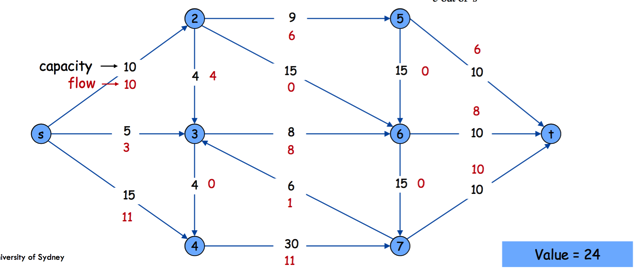
\includegraphics{images/Week_9/FlowNetwork.jpg}
  \caption{Flow network.}
  \label{FlowNetwork}
\end{figure}
from this, we want to know what is the \textbf{maximal flow} of the network. We can notice that cutting the network can give us the optimal flow.


\textbf{s-t cut} is a partition (A,B) of V with s $\in$ A and t $\in$ B. Here, we cut the graph into A and B, where the source is in A and the sink is in B. The \textbf{capacity} of a cut(A,B) is defined as: $cap(A,B) = \sum_{\text{e out of A}c(e)}$ . Here, the capacity of the cut is the summation of the \textbf{capacity of the edges going \underline{out} of A}

From this, we can define the famous lemma:
\begin{center}
  \textbf{Flow value lemma: } Let f be any flow and (A,B) be any s-t cut. The net flow sent \textbf{across the cut} is equal to the amount leaving s.

  v(f) = $f^{out}(A)$ - $f^{in}(A)$
\end{center}
Recall that v(f) is the value of the flow leaving the source node. Intuitively, whenever we make a cut, the net flow that is leaving from A into B, has to equal to the flow that comes directly from the source vertex. This flow needs to go through the graph and therefore needs to be passing through any cut we make in the graph.

\begin{center}
  v(f) = $f^{out}(A)$ - $f^{in}(A)$

  Value of the flow from the source is equal to the netflow leaving A/going across the cut

  v(f) = $f^{out}(s)$ - $f^{in}(s)$

  The value of the flow from the source is simply the out flow from the source and can be rewritten as the net flow from the source (but remember that the inflow into the source is 0)

  By the flow conservation, the net flow for every vertex, except for the source vertex, is 0.

  This means that

  $f^{out}(v)$ - $f^{in}$ = 0 for all vertices.

  This brings us to:

  = $\sum_{\text{v in $\in$ A}}(f^{out}(v) - f^{in}(v))$

  so for every vertex in A, the netflow is the flow coming out of the vertices in A net of the flow coming into the vertices in A.

  = $\sum_{\text{e out of A}}f(e)$ - $\sum_{\text{e into A}}f(e)$

  This is looking at the flow for each edge coming out of A net of the flow for each edge coming into A. Therefore we arrive at:

  = $f^{out}(A)$ - $f^{in}(A)$
\end{center}

\textbf{Weak duality:} Let f be any flow and let (A,B) be any s-t cut. Then, the value of the flow is \textbf{at most} the capacity of the cut due to the principle that flows can't exceed the capacity of edges, which means the total flow can't exceed the total capacity in the s-t cut.

\begin{addmargin}[1em]{2em}% 1em left, 2em right
\textbf{Proof: }
\begin{center}
  v(f) = $f^{out}(A)$ - $f^{in}(A)$

  The value of the flow is equal to the net flow across the cut s-t from flow value lemma.

  $f^{out}(A)$ - $f^{in}(A)$ $\leq$ $f^{out}(A)$

  The net flow has to be at most the flow coming out A and across the cut s-t. This can be expressed as:

  $f^{out}(A)$ = $\sum_{\text{e out of A}}f(e)$

  which equals to the flow coming out of each edge in A.

  v(f) $\leq \sum_{\text{e out of A}}f(e)$

  which has to be at most the \textbf{capacity of the edges coming out of A}.

  v(f) = c(A,B) $\square$
\end{center}
\end{addmargin}

\textbf{Corollary: }

Let f be any flow and let (A,B) be any cut. If the value of the flow v(f) is equal to the capacity cap(A,B), then f is a max flow and (A,B) is a minimum cut. Note that f is just a flow whilst v(f) tells us what the \textbf{actual value} of the flow is. Recall that cap(A,B) is the capacity of the outgoing edges from the set A.
\begin{center}
  Therefore, if v(f) = cap(A,B), then f is a max flow and (A,B) is a min cut.
\end{center}

\textbf{Theorem: } Maximum flow $\leq$ minimum cut

\subsection{Max Flow algorithm}
From the previous section, we can now start designing a way such taht given a flow network, how can we arrange traffic to make as efficient use as possible of available capacities. Therefore, given a flow network, we want to t find a flow of maximum possible value.

From this, every time we make a s-t cut to partition the network into 2 sets A and B, such that s $\in$ A and $\in$ B, we can arrive at the following conclusion. Any flow that goes from s to t, must at some point cross from A into B and therefore utilise the capacity of the edges going from A into B. This means that such a s-t cut, puts an upperbound on the maximum possible flow value. From this, we can see that the smallest capacity edge going from A into B, will be the maximum flow we can push from s into t.

We can see that from this a greedy algorithm will not work in this scenario as this will satuarate the paths and since we can't backtrack on previous solutions, will lead to an inefficient solution.

What we will need is a \textbf{residual graph} $G_{f}$ = (V,$E_f$). The vertex set in $G_f$ is identical to the vertex set in G.

Furthermore, ff we have an edge e = (u,v) $\in$ E with a flow f(e) and a capacity c(e), we can create a \textbf{residual edge}. We can refer to the below figure.

\begin{figure}
  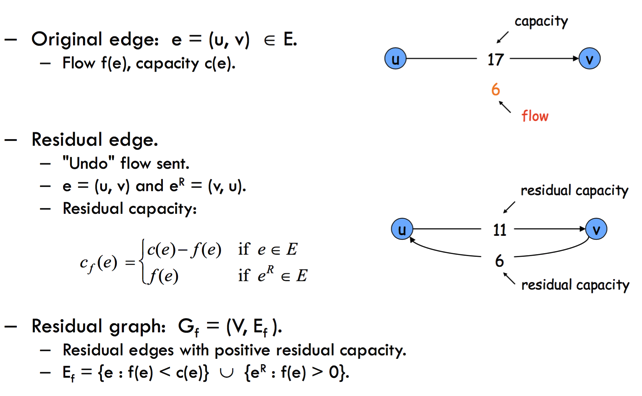
\includegraphics[width=\linewidth]{images/Week_9/ResidualEdge.jpg}
  \caption{Edge and Residual Edge}
  \label{ResidualEdge}
\end{figure}

To construct a residul edge, we \textbf{undo} the flow sent. What this means is that for each edge e=(u,v) in G, where the flow f(e) < c(e), there are $c_e$ - f(e) leftover units of capacity to push more flow forward. Therefore we can construct a \textbf{forward edge}. So if e=(u,v), then $e^{r}$=(v,u), so we swap the direction of the edge. Furthermore, we create a backedge which has the capacity of e whilst the forward edge has a capacity c(e) - f(e). For each edge e = (u,v) of G whereby the flow f(e)>0, then there are f(e) units of flow we can undo by pushing backwards. This is why we include it in our residual graph $G^f$ as a backward edge.

From this, the residual graph $G_f$ = (V,$E_f$) has residual edges with positive residual capacity. Here, in $E_f$, it comprises of 2 parallel edges: one wiht a flow less than the capacity constraint and another with a flow greater than 0. Doing this, undoes the flow sent.

The \textbf{residual capacity} of an edge in the residual graph $G_f$ tells us how much flow we can still send, given the current flow. Therefore, the residual capacity tells us the capacity of the edges in the residual graph $G_f$.

Let P be a simple s-t path from the source vertex s to the sink vertex t \textbf{in the residual graph $G_f$}. Furthermore, we can define the \textbf{bottleneck(P,f)} to be the minimum residual capacity of any edge on P with respect to the current flow f. Pretty much, if we have a path from s-t, the bottle neck is the edge with the smallest capacity.

We can now define the pseudocode for \textbf{augmentation}:

\begin{algorithm}
\caption{Augmnetation}\label{euclid}
\begin{algorithmic}
\Procedure{Augment(f,p)}{}
\State $\textit{b} \gets \text{bottleneck(P,f)}$
\State \emph{for each e = (u,v) $\in$ P \{ }
\If {\textit{e is a forward edge}} \State increase f(e) in G by b
\Else {\textit{ e is a backward edge}}
  \State decrease f(e) in G by b
\EndIf
\State \}
\BState $\textit{return f}$
\EndProcedure
\end{algorithmic}
\end{algorithm}

What this augmenting algorithm does is, we find a path from s-t. A path means that each vertex is only visited once in our path. From this, we look at the bottleneck in our path (or the edge with the smallest capacity). The bottleneck(P,f) is the minimum residual capacity of any edge on P, with respect to the flow f. If the edge in our residual graph is a forward edge, we can simply increase the flow in our original graph G going throuugh that edge by b. If the edge is a backward edge, we decrease the flow in our original graph by b. This Augment(f,P) algorithm gives us a new flow f' in our original graph G by increasing or decreasing the flow values on edges of P. Any s-t path we analyse in the residual graph $G_f$ is known as the \textbf{augmenting path}.

\subsubsection{Ford-Fulkerson Algorithm}
From what we've done so far, we can now utilise the idea of augmenting paths to determine the maximum flow.
\begin{algorithm}
\caption{Max-flow}
\begin{algorithmic}
\Procedure{Ford-Fulkerson(G,s,t)}{}
\ForEach {$e \in E $}
\State $f(e) \gets 0$
\State $\text G_f \gets \text{Residual Graph}$
\EndFor
\While {there exists augmenting path P in $G_f$}
  \State $\textit{f} \gets \textit{Augment(f,P)}$
  \State $\text{update $G_f$}$
\EndWhile
\State \}
\BState $\textit{return f}$
\EndProcedure
\end{algorithmic}
\end{algorithm}

Initially, we set all the flows to 0 and we construct a residual graph $G_f$. When there is still an augmenting path P in the residual graph $G-f$, what we do is we augment the path and return the flow. We find the minimum residual capacity of the path. We then update the residual graph $G_f$. We can use BFS to locate the augmenting path. Finally we return the flow. When we augment a path, we look at whether the edge in our path in the residual graph is a forward or backward edge. If it is a forward edge, we then update our original graph's edge by increasing f(e) by b else it is a backward edge we are looking at so we decrease the flow in the original graph G by b. Refer to lecture slides page 32 onwards for an actual example of this algorithm in pracitce. We stop augmenting the path when there is no longer a path from s to t in the residual graph. At the end, we can take the minimum s-t cut, which will be equal to the max flow. In the residual graph, we do this by placing into set A, all vertices that are reachable from s. Then going back to the original graph G, we can look at either the \textbf{outgoing capacity} of the edges from the set A OR the \textbf{net flow} from set A into set B. The capacity of outgoing edges from A is equal to the netflow outgoing from A. This gives us our max flow.

So when we augment a path in the \textbf{residual graph}, if in the residual graph, the edge is a backward edge (which means it points to a different direction compared to the edge in the original graph), then in the original graph G, we then decrease the flow by the bottleneck. If the edge in the residual graph for our augmenting path is a forward edge, we then just increase the flow of that edge in the original graph by the bottleneck.

\subsubsection{Analysis}
\textbf{Assumption:} We assume all initial capacities are integers.

\textbf{Lemma:} At every intermediate stage of Ford-Fulkerson algorithm, the flow values and the residual graph capacities in the residual graph $G_f$ are also integers.

\textbf{Proof by induction:}
\begin{addmargin}[1em]{2em}% 1em left, 2em right
Base case: Initially the statement is correct before the while loop.

Induction Hypothesis: It is still true after j iterations.

Induction Step: Since all residual capacities in $G_f$ are integers, the bottle-neck value must also be an integer. Therefore, the flow will have integer values and also the capacities will have integer values in the new residual graph.
\end{addmargin}

\textbf{Integrality theorem:} If all capacities are integers, there exists a max flow f for which every flow value f(e) is an integer.

We can use this property to prove that Ford-Fulkerson algorithm terminates.

\textbf{Augmenting Path Theorem:} Flow f is a max flow iff there are no augmenting paths.

\textbf{Max-flow min-cut theorem:} Value of max flow is equal to the value of the minimum cut.

\textbf{Proof}
\begin{addmargin}[1em]{2em}% 1em left, 2em right
We have 3 things to note

(i) There exists a cut (A,B) such that there is a flow v(f) = cap(A,B)

(ii) Therefore, flow f is a max flow

(iii) There is no augmenting path relative to the flow f
  \begin{addmargin}[3em]{4em}
    (i) implies (ii) due to the corollary of the weak duality lemma since the value of a flow is at most the capacity of the cut (A,B)\\

    (ii) implies (iii) by a simple proof. Let f be a flow, if there exists an augmenting path, then we can still improve f by sending flow along a path P and then augmenting the flow G. Therefore, there can never be no more augmenting paths relative to f or else f is not the max flow and we can still improve upon it.

    (iii) implies (i) which is the \textbf{proof of Max-Flow Min-Cut Theorem}. Let f be a flow with no augmenting paths. Let A be the set of vertices that can we reach from the source s in the residual graph. Recall that source s is an element of set A whilst sink t is an element of set B.
    \begin{center}
      $v(f) = \sum_{\text{e out of A}}f(e) - \sum_{\text{e in to A}}$

      $= \sum_{\text{e out of A}}c(e)$

      and since there is no augmenting path from A to B

      $= cap(A,B)$
    \end{center}
    Here, the value of the flow is the netflow from A into B. However, since there are no longer any augmenting paths, the outgoing capacity is equal to the netflow from A into B. Therefore, the value of the flow is equal to the capacity.
  \end{addmargin}
\end{addmargin}

\textbf{Observation:} Let f be a flow in G and leet P be a simple s-t path in the residual graph $G_f$. The \textbf{flow value strictly increases in augmentation}.
\begin{center}
v(f') = v(f) + bottleneck(f,P)

The new flow value is the summation of old flow value and the bottleneck. The first edge e of P must be an edge coming out of s in the residual graph and since P is a simple path, vertex s is not visited again. Since G has no edges entering s, then edge e \textbf{must} be a forward edge. From our augmentation algorithm, we can only ever increase the flow of this edge.

Since the bottleneck(f,P) $>$ 0, this implies that

v(f') $>$ v(f)
\end{center}

We can also define the notation
\begin{equation}
  C = \sum_{\text{e out of source s}}c(e)
\end{equation}

\textbf{Observation:} C is an upper bound on the maximum flow. The maximum flow cannot be greater than the flow coming out of the source vertex.\\

\textbf{Theorem:} The algorithm terminates in at most v($f_{max}$) $leq$ C iterations. So we can only run this at most C iterations.

\textbf{Proof:} Each augmentation increases the flow by at least a value of 1. It can only be at most C iterations since the flow value can not exceed the capacity coming out of the source vertex C.\\

Let n denote the number of vertices and m denotes the number of edges in graph G. Since each node has \textbf{at least} one incident edge, therefore m $geq$ $\frac{n}{2}$ since each edge is connected to 2 vertices. Therefore, we can bound O(m+n) = O(m) since O(m+2m) = O(m).\\

From this, Ford-Fulkerson runs in \textbf{O((m+n)C) time} or \textbf{O(mC))} time if all capacities are integers (whole numbers).

\textbf{Proof:}
\begin{addmargin}[1em]{2em}% 1em left, 2em right
  We know Ford-Fulkerson runs in at most C iterations.

  The residual graph $G_f$ has at most 2m edges compared to the original graph G. We can maintain $G_f$ using an adjacency list representation whereby we have 2 linked lists for each node $v$. One list contains the edges entering $v$ and the other list contains edges leaving $v$.

  In each iteration, a path in the residual graph $G_f$ can be found in O(m+n) using BFS. Since m $geq$ $\frac{n}{2}$, this can be simplified down to O(m).

  Augment(P,f) takes O(n) time to traverse through the simple path with at most n-1 edges.

  Given the new flow f', we can update $G_f$ in O(m+n)/O(m) time whereby for each edge e of G, we construct the correct forward/backward edges in $G_f$.
\end{addmargin}

From this, O(mC) is only decent if C is small. The issue is that Ford-Fulkerson is not polynomial in terms of input size (m, n, and logC). The reason is that if we were given a flow, the total iterations taken by the algorithm will depend on the max capacity D. Let us say that D = 100 but however, there is an edge capacity in the graph with a capacity of 1. Using an augmentation algorithm, we will slowly increment the flow by 1 each time until we finally reach our capacity of 100. This will take a long time and be inefficient. Refer to slide 50 in lecture for a better explanation.

From this, we need to choose better augmenting paths.\\

\textbf{Goal:} Choose augmenting paths so that:

- Can find augmenting paths efficiently.

- Take less than C iterations to run.

\subsection{Edmonds-Karp Algorithm}
We can use the Edmonds-Karp algoritm in order to find better augmenting paths. The current possibilities of choosing augmenting paths are:

1) Ford Fulkerson - Choose any augmenting paths (C iterations)

2) Edmonds Karp 1 - Choose max flow path (mLogC iterations)

3) Improved Ford Fulkerson - Choose max flow path (log C iterations)

4) Edmonds Karp 2 - Choose minimum link path (O(nm) iterations)\\

\subsubsection{Edmonds-Karp 1}
Here, we pick the augmenting path with the largest capacity in order to maximise the bottle neck picked. We pick the path with the maximum minimum capacity.

\textbf{Claim:} If maximum flow in G is F, there exists a path from s to t with capacity of at least $\frac{F}{m}$

\textbf{Proof:}
\begin{addmargin}[1em]{2em}% 1em left, 2em right

Delete all edges of capacity less than $\frac{F}{m}$ and we can see that the graph is still connected. This is because if you think about it, the remaining graph must have a path from s to t. Since the edges have a capacity of at least $\frac{F}{m}$, the path itself has a capacity of at least $\frac{F}{m}$.

\end{addmargin}

\begin{center}
  LOOK AT PROOF AGAIN ON PAGE 22 IN COMP2907 WEEK 11 LECTURE.
  \textbf{Edmonds-Karps 1 takes at most O(mlogF) iterations.}
\end{center}

\subsubsection{Improved Ford Fulkerson}
Instead of finding max flow path, we find an approximate max flow path by \textbf{capacity scheduling}. Run same FF algorithm but run it on subgraph of the residual. We don't need global bottleneck but we want to ensure that the path we find is still pushing through alot of flow (doesn't have to be the highest flow). We keep a sclaing parameter and build a residual graph with scaling paramter. This subgraph is the subgraph with arcs containing capacity of at least $\Delta$. When we find the augmenting path, it must finds the capacity that is at least bigger than $\Delta$.

\textbf{Pseudocode for capacity scaling}

Set $\Delta$ to initial value that is related to C. Build residual graph and do iterations.

We start removing all edges smaller than $\Delta$ and then we find an augmenting path in the $\Delta$ bounded residual graph and update the flow in the original graph with the bottleneck capacity which has to be bigger than $\Delta$. When we can't find any more paths, we decrease $\Delta$ and repeat the algorithm again with a smaller bounded path. When $\Delta$ is 1, we end back at Ford Fulkerson so we have no difference between this and Ford Fulkerson.

\textbf{Runtime}


We perform iterations LogC number of times for the outer while loop. Updating residual graph is O(m) since m $\geq$ n-1.

For the inner while loop, it is harder to see how many loops we do. If we fixed delta and look at only one iteration of $\Delta$ value of the flow increases by at least $\Delta$ in each iteration. Value of flow is v(f) + m$\Delta$. This means that we are dividing $\Delta$ by 2 but we can only increase it by at most 2m$\Delta$.

Let A be source of vertices we can reach from source and B theo ther set. Flow is net flow going into B and coming out of B. We can then rewrite the equation as:

c(e) $leq$ f(e) + $\Delta$ since if this is not true, then we would have an edge in residual graph from A-B since residual capacity of the edge is the capacity of the edge minus the flow f(e). This edge does not exist in $\Delta$ graph so that means the flow must be less than $\Delta$ or else it wouldn't be in there in the first place.

c(e) - $\Delta$ = f(e) which we can sub in to the formula.

If f(e) > $\Delta$, then we would have a forward edge which we shouldn't have.

Everything goes out of A is the capacity of the cut. Furthermore, all the edges going out of A and all edges going into A, is upperbounded by m. This means that the remaining flow cannot be huge and decrease in each phase.

Therefore the while loop runs in 2m runtime.


\subsubsection{Edmonds Karp 2}
This runs in nm iteration. Does not look for path of max flow, it just looks for path of minimum number of links. We use BFs to find path with number of least edges.

\textbf{Proof of runtime}

Uses 2 observations. Let d be number of links in the augmenting path from s to s in current residual graph.

1) We then augment that flow and the observation is that this distance will never decrease. It will only ever increase or stay the same.

\textbf{Proof}
Consider the BFS levels from s to t. Each iteration of BFS will give us levels. We find the augmenting path from s to t and need to stop at a vertex in every level. When we find the path, we augment the flow in the residual graph. Along this graph, we have a bottleneck and this edge's residual capacity will become 0 and become a backward edge. Now there is no new path from source to sink that has a less length than the path we just created. It becomes a backward edge since bottleneck capacity is equal to the residual capacity of the edge so which causes it to become a backward edge. Therefore, we can't take this path anymore and need to find a new path via BFS, which will be longer since BFS will always find the path that is shortest first.

2) If we perform m iterations, then the distance d from s to t has to increase by at least 1.

\textbf{Proof}
After every iteration, we are going to flip at least one forward edge and turn it into a backward edge. We can only do that m times. After we flipped all the edges, then the distance has to increase by at least 1.


From this, we know Edmonds-Karp performs at most nm iterations and does not depend on the capacity in order to run it.

\subsubsection{Section Overview}
\textbf{Augmenting Path Theorem:} Flow f is a max flow iff there are no augmenting paths in the residual graph.

\textbf{Max-flow Min-Cut Theorem:} The value of max flow is equal to the value of the min cut.

\textbf{Integrality}: If all capacities are integers, then every flow f(e) and every residual capacity $c_{f}(e)$ remains an integer through the algorithm.

C is an upper bound on the maximum flow where by: $C = \sum_{\text{e out of s}}c(e)$

Ford-Fulkerson runs in O(Cm) time.

\subsection{Flow Network Applications}
We have alot of problems which we can rewrite into a maxflow problem which will be equivalent to solving the original problem.

\subsubsection{Bipartite Matching}
We are given an \textbf{undirected graph} G = (V,E). We can say that set matching M whereby M $\subseteq$ E if each node appears in at most one edge in M. We want to find the \textbf{maximum cardinality matching}. This means that we want to find the matching with the most number of edges whereby every vertex is incident at most one edge. We can recast this problem as a bipartite matching. This gives us a bipartite graph. Bipartite graphs has the vertices divided into 2 sets whereby edges are across the sets. There are no edges within the set and every edge therefore straddles between the 2 sets. A \textbf{matching} is when each node appears in at most one edge in M. From this, we want to find a maximum cardinality matching. We want to find maximum matching of bipartite graphs whereby each vertex in the sets are connected by only 1 edge to a vertex in the other set.

\textbf{Max Flow Formulation}

We can formulate this by transforming the undirected graph G into a digraph G'. This disgraph G' = (L$\cup$R$\cup$\{s,t\}, E').  We direct all edges in G from L to R. We can then add a node s, and an edge (s,l) to each node in L from s. We can also add a sink node t and create edges (r,t) whereby we have an edge from each node in r to point at the source t. Finally, for our digraph itself, we assign an edge capacity of 1 for each node in L pointing to R.
We need to prove that maxflow of the graph is equivalent the value of the maximum cardinality matching in G. \textbf{We need to prove this in both directions}.

\textbf{Proof that maximum cardinality matching in G is the max flow in G'}

Assume we have a max matching M with a cardinality of k. We have k edges and sending out a flow along these k paths. Since f(e) = 1 for each path, this will give us a flow f in s-t flow of value k. If k edges in maximum matching, there will be a flow of value k. This only proves that if cardinality matching of size k, then there is a flow of value k. This does not say if max flow is k, then max cardinality is k. We need to prove the other direction.

\textbf{Proof that value of max flow in G' is the maximum cardinality} Let us say we have a maxflow k in G'. We need to use the fact that we only have integers. Due to integrality theorem, we know every edge has a flow of 0 or 1. We look specifically at edges between left and right set has an edge of capacity 1. Due to conservation property, each vertex can only have one unit of flow coming into the vertex since the edge from vertex to sink has a capacity of 1. We consider the set M' of edges of the form (x,y). M' contains k edges.

Runtime of this algorithm:

N vertices on left side and N vertices on right side. We have at 2N + M edges in our graph (N vertices from sink and N from source). Then we have M edges between left and right set. Algorithm runs in O(mn).

\subsubsection{Perfect Matching}
Each node only needs to appear in one edge. First we require that there are the same number of vertices in both sides. If we pick 3 vertices on the left side, then we must have 3 neighbours on the other side. Therefore, if we have a subset S, and we look at neighbours of that set N(S), if there is a perfect matching, then for every subset of S, the number of neighbours in S has to be equal or greater than number of vertices in subset S. This holds for all sets S.

It is true the other way too.

\textbf{Marriage Theorem}: If we have a bipartite graph and equal number of vertices in both side. G has perfect matching if for every subset S the number of neighbours is equal or greater than set S. If there is no perfect matching, then this does not hold.


If no perfect matching, flow is less than n. If flow is n, then we can connect each vertex in left to vertex in the right. By max flow min cut theorem, if flow smaller than n, then min capacity  is smaller than n.

Suppose we have a set $L_a$ with just 2,4,5 on slide 28. Neighbours to $L_a$ is just the 2 vertices 2' and 5'. We can make A a bit bigger and the cut bigger but we won't change the capacity of the cut. We move the neighbours of the set 2' and 5' into the set $L_a$. We move the neighbours of $L_a$ into $L_a$. Now when we include 2' into $L_a$, we have only 1 new edge which is from 2' to t which is our new cut. The edge between 2 and 2' is no longer in the cut. We increase the cut by 1 edge but we also decrease the cut by 1 edge. Therefore, the capacity does not increase as a result. So now we can include both neighbours $L_a$ into A. Now looking at the capacity between A and B, there are only 2 sets of edges that will contribute to the cpaacity. From S, we edges that will go to a vertex that goes outside of A, all the vertices on left side but not in A. LnB means vertices on the left that belongs to B. We also look at vertices on the right side that belongs to the set A. We took all the vertices that belongs in left side that belong to A and its neighbours are also in A so these aren't connected to things not outside of A. Number of vertices in right side that belong to A, are at least all the neighbours of $L_a$ we just put into A. No perfect matchign so maxflow is smaller than n, so min capacity and max flow are both below n. Capacity of A and B can give us the stuff we just derived on slide 34. In the end, number of vertices in $L_a$ is greater than the number of neighbours in $L_a$.

\subsubsection{Disjoint Paths}
Given a directed graph and source/sink nodes, we want to find the maximum number of edge-disjoint s-t paths. We want to find number of paths that don't use the same edge (but can use the same vertex).

We want to find how many \textbf{edge-disjoint} paths there are. We want to turn this into maxflow problem and say that the max flow is the optimal.

We assign unit capacity to every edge.

We want to prove max number edge-disjoint s-t paths equal max flow value.

Suppose K $P_k$ paths. Set the flow of an edge f(e) = 1 if edge participates in some path. Since these paths are edge disjoint, then each path will transport value of 1. Therefore, the flow of this network will have a value of k.

For the other direction, assume max flow is k. If max flow is k, number of edge disjoint paths is of value k. Amount of flow going through edge either 0 or 1. We continue choosing a new edge until we reach the sink, producing k disjoint paths.

This shows us both directions and therefore maxflow is number of edge disjoint paths.

\subsubsection{Network Connectivity}

This is used for \textbf{fault tolerance}. How many connections we have to break in order to disconenct the graph. Network connectivity is when We want to find the number of edges to disconnect the source from the sink. A set of edges F disconnects t from s if all s-t paths uses at least one edge in F.

\textbf{Theorem}: Max number of edge-disjoint s-t paths is equal to the min number of edges whose removal disconnects t from s.

\textbf{Proof}: Suppose removing set k edges, we get 2 components now. Any path from s-t has to use at least one of the edges from k. If not, then s can use that path to reach t and therefore it is still connected.

Assume max number of edge disjoint paths is k. If we remove k edges, we disconnect the set. K edge-disjoint paths and therefore we know the maxflow is k. If max flow greater than k, this generates new augmenting path. If max flow is k, there exists a min cut of k. We look at the min cup with capacity k. Let F be set of edges that straddles the (A,B) cut. Let $|$F$|$ = k and we have exactly k edges going from A to B.

This reduces to finding max flow.

\subsubsection{Circulation}
Directed graph G = (V,E). The edge capacities c(e), where e $\in$ E. We have one new thing now, every node has either a supply or a demand. We have all these nodes and vertices and they produce stuff. They supply something or demand something. Can we create a flow that fulfils all the supply, demand, and capacity. 0 means we don't produce anything. Supply is negatiev. Demand is positive.

\textbf{Circulation}: We have a capacity constraint and conversation constraint. However, conservation criteria is different since what goes into a vertex - what goes out, equals to the demand or supply of that vertex. We are given all these parameters and we want to know does there exist a circulation that makes everyone happen. We want to model this as a flow network problem. We can think of us having multiple source and sink nodes now.

\textbf{Necessary Condition} Sum of supplies = sum of demands. Necessary condition is sum of supply equals sum of demand.

For a supply vertex, the outgoing is the incoming flow + the supply of the vertex. These vertices with a supply has a flow that goes out from them that is exactly the supply value.

We make a super source and super sink. We create a new vertex source whereby it has an edge to each supply vertex with edge capacity of the supply. We then do the same for a super source where we connect super source to all demand vertices and create edge capacities with demand.

Using the integrality theorem, if all capacities and demands are integers, there exist a circulation than all of them are integers too.
If everything is integers, then everything and the solution will also be integers. There exists a feasible circulation with demand $d_v$ iff for all cuts (A,B).

\subsubsection{Circulation with supply/demand and lower bounds}

Instead of saying flow has to be nonnegative and upperbounded, we can now say we have a new lower bound. If all values are integers, then the circulation value will also be integers and we can model this as a flow network too.

\subsubsection{Survey Design}
Design a survey with $n_1$ consumers and $n_2$ products. We can only ask question about consumer i about product j if they own it. We ask consumer i a certain number of questions (at least $c_i$). Each product gets a least a certain number of reviews $p_j$. We want to design a survey to meet these specifications.

We set of consumers on the left and set of products on the right. We formulate as a circulation problem with lower bounds. Include an edge if the consumers owns that product. Each consumer has to review a number between $c_1$ and $c_1$' items. We want to model it as an integer circulation so we have one edge from sink to source with capacity of infinity. If there exists an integer circulation, this corresponds to a feasible survey. If circulation problem with lower bounds is feasible, then survey design problem is feasible.

\subsubsection{Image Segmentation}
A picture of just pixels is given to us. We to identify the foreground and the background. We have a picture of $nxn$ set of pixels. We preprocess the image and have a likelihood that the image is in the foreground or the background. We can't just look at a single pixel, we need to look at neighbouring pixels too. If we classify a pixel in the foreground, then its more likely the neighbour is also in the foreground too. If we have 2 pixels where one is in the background and one in the foreground, we have to pay a penalty for that. We want to minimise the penalty for that. We want to find a partition (A is foreground and B is background) and we want to maximise the summation of a, b, and negative of this penalty function. If 2 vertices belong to 2 different set, we need to pay the penalty for this. A and B are not influenced by since we preprocessed likelihood in the beginning.

Here we want to maximise the cut. So what we can do is rewrite the objective function s.t. we are minimising it. We take all the a and b values - all the a values in a and b values in b. We add a penalty function too. This is from the duality problem. Therefore, we want to minimise the sum of A values in B, sum of B values in B, and the penalty function.

We want to model it as a flow network with a source and sink added. We add a source and a sink. For every incident pair of vertices, we add a capacity $p_{ij}$ edge going both ways between them. Then we add an edge from source to every pixel with value $a_j$. We edge from vertices to sink with capacity $b)i$.

Min cut now must contain source in A. Value of the mincut is all the edges from the source to all the vertices in b (sum of all a values for every value in b). 3rd time is all the penalty functions so for every edge pair, one vertex lies in a and the other in b, which means the penalty of that edge is the penalty term.

\subsubsection{Baseball Elimination}
We don't care about the losses, only the wins. We want to look at wins, how many games left to play, and who they will play.

Say we want to model whether can team 3 win. The edges go from the source to all possible games. Source to first vertex, means that those 2 teams will play that many. Since integer setting, we split that up by integers. $r_3$ is the number of games they can win.

\newpage
\section{NP Hardness}
We are looking at what problems are hard.

Reduction: How you reduce one problem into another problem in polynomial time. There are 3 classes for reduction that are quite famous. If we have a problem that can be solved in polynomial time, then we believe we can solve it in practice. Problems that are in exponential in nature, it is unlikely we can solve them in practice. There are a few problems we have solved in polynomial time. However, there are quite a few problems we have not solved in polynomial time such as the finding the longest path in a graph or finding a max cut.

\textbf{Aim}: Classify problems we can solve in polynomial time and those we can't solve in polynomial time. However, we don't know how to do this. Alot of problems that we don't know that are hard problems, can all be reduced down to one problem. If we can reduce this into its 1 problem and solve it, then we can solve all problems.

\subsection{Polynomial time reduction}
For assignment 4, if we can solve max flow in polynomial time, then we can solve the schedule tree in polynomial time too.

The reduction says that the problem X can be transformed into problem Y in polynomial time. If every instance of X can be solved by

- Polynomial number of standard computational steps (transforming X into something we want).

- We can call algorithm for problem Y for a polynomial number of times.

\textbf{Example}: Computing transitive closure of a directed graph. We can compute the BFS tree from every vertex. So starting from A, what vertices can we reach from A and then add an edge between them. Doing N BFS calls, we will be able to extract the transitive closure. This is a polynomial time reduction.

So the steps to do these problems are:
\begin{center}
  1) Transform X into Y.

  2) Solve it for problem Y with an algorithm.

  3) Then we collect the output from stage 2 and then we merge it into 1 solution for problem X.
\end{center}

The transitive closure of the polynomial reduces to BFS in computing the transitive closure of a graph. The number of times we make a call to BFS is linear.

1) \textbf{Design algorithms}: Since we can solve Y in polynomial time, then we can solve X in polynomial time.

2) \textbf{Establish intractability}: If X can't be solved in polynomial time, then Y cannot be solved in polynomial time. This is because transformation from X into Y is polynomial time.

If we say X polynomial reduces into Y, and Y polynomial reduces into X, then we can say that there is \textbf{equivalence}.

\textbf{3 most basic types of reductions}

\subsection{Reduction by Simple Equivalence}
Here, we have an \textbf{independent set} where given a graph G and an integer k, is there a subset of the vertices containing at least k vertices such that each edge, one of its endpoint is in the independant set. Every vertex has at least one edge in the independent set. We don't vertices that are connected to each other via an edge So for the example, we have an independent set of at MOST size 6. \textbf{Vertex cover} is such that with k vertices, all the edges in the graph is adjacent to one of the k-vertices. Just pick vertices that aren't connected by same edge.

\textbf{Decision problem}: Every algorithm is going to be a yes or no question. So does there exist an independent set of size at most k.

Search problems are optimisation problems of the decision problems. The \textbf{search problem} can be reduced to the decision problems in this course.

The complement of the independent set is the vertex cover.

\textbf{Vertex Cover}: Each edge is connected to a vertex in the set s.

VERTEX COVER SEEKS TO FIND MINIMUM NUMBER OF VERTICES REQUIRED TO CONNECT TO ALL EDGES IN THE GRAPH. INDEPENDENT SET JUST WANTS VERTICES THAT AREN'T LINKED BY AN EDGE.

Solving vertex cover in polynomial time lets you solve independent set in polynomial time too. There are equivalent.
\textbf{Proof}
$\leftarrow$ proof
We have v - s set of vertices. We look at two vertices in S. There can be no edges between these 2 vertices because if there is, then there should be in the vertex cover.
Vertex covering reduces to independent set and independent set reduces to vertex covering.

\subsection{Reduction from special case to general case}
Most common way. If we have a general case and then we do a reduction from a special case into a general case. We have a reduction from vertex cover to set cover. \textbf{Set cover} if we are given a universe collection of elements and k. Does there exist a collection of k of these sets whose union is equal to U. We have a shopping list of k and each shop can generate a subset of items. We want to go to minimum number of shops to buy all the stuff on our shopping list.

By taking the union of set 2 and set 6, we get the items of the universe. Here we can double up.

Vertex cover: For every edge, one of its vertices has to be in the vertex cover. We can do a reduction from vertex cover to set cover. Vertex cover is a special case of the set cover.

We want to look at if theres a vertex cover of size 2 (k=2). My universe is the set of the edges (we have 7 edges). We want to see to it, that for every edge, one of its end points is in the vertex cover. If we pick a set, that corresponds to picking a vertex. Generate one set for each vertex and items we put into that set is all the incident edges. So set of edges for vertex f, is e1,2,6, and 7. So now we can rewrite vertex cover as set cover. Looking at set cover solution, we pick f and c. Here, every edge is covered by f and c. (Every edge is connected to a vertex).

\subsection{Reduction via Gadgets}
We can also reduce via \textbf{gadgets}. A sat problem is quite important. We have a literal which is a boolean variable (so either itself or NOT itself). Clause is a disjunction of literals so x1 not x2 or x3. Putting all these clauses together using conjunctions, So clause c1 and c2 and c3 and c4. Can we assign boolean values to the variables such that the formalised is satisfied?

3-Sat is whereby for each clause, you can have only 3 literals. (3 boolean variabels in each clause). Is there a literal assignment such that the CNF is true. Set x1 to true, clause 2 and 3 are true. Set x2 to true sets clause 1 and 3 to be true. Set x3 to false, then clause 4 is true now. Therefore we can assign a truth assignment.

\textbf{Proof that 3-set reduced as independent set}:
Independence set ask for if there is a set of size at least k, then each end point is in S.

We can a CNF formula of 3-SAT. The instance for independent set is a graph. We want to show that the independent set will be a yes instance iff formula is satisfied.

We get the 3-SAT problem as input and build our graph G whereby we have 3 vertices for each of the k clause. For each clause, we build these 3 vertices. Each vertex will correspond to a literal in that clause. Then we do the same thing for next clause. Then connect 3 literals in each clause into a triangle. We add these edges because we are computing the independent set. If we pick one of these edges, we can't pick any of the other edges. This forces us to pick one edge from each triangle. We can pick one from each triangle. We can to also prohibit NOT choosing both x1 and not x1. Therefore, we can add an edge between x1 and not x1. We do this for every variable that are complements of themselves. This forces us to pick only x or not x. Now we run our independent set algorithm and will give us an independent set. If there exists an independent set that can pick 1 from each clause and pick k vertices, then the SAT instance will be a yes. We can pick at most 1 from each triangle. If we don't pick 1 from a triangle, then the clause will be false. If we can pick 1 vertex from every triangle, then we have k. If we can pick k therefore we get a truth assignment to the 3-SAT.

\textbf{Proof}
Suppose S is an independent set of size k whereby s must contain exactly one vertex in each triangle. We set these literals to true and therefore truth assignment is consistent and all clauses are satisified. For the other way, if we have a satisfiying assignment, then we can pick one true literal from each triangle and therefore we have an independent set. Having an algorithm for independent set means we have a 3-Sat problem.

\subsubsection{Clique}
Clique of graph G is a complete subgraph of G. We have a complete subgraph of size 4.

We make a column for each of the k-clauses. We have no edges between 2 vertices within a column. We have a complete graph except between every literal x and its negation.

We put first clause into first column (layer). Then each clause for each column. THE LAST CLAUSE SHOULD HAVE 3 LITERALS IN IT. No edges between a literal and its negation in this graph. Can we have 2 vertices in the same column for a clique because we have no edges between vertices in the same column. Therefore if we have a k-clique, then it will contain 1 vertex from each column. Each literal is connected to all other vertices except the negation of itself. So if there exists a k-clique, then it has to be connected to exaclty 1 literal in the column and cannot be connected to the negation of itself. If we pick the set X,Z,Y then the first clause is true (x is true) and Z is true (2nd clause is true) and Y is true means that the 3rd clause is true.

We also have the property of transitivity too.

\subsection{NP}
REWATCH LECTURE!!!

\textbf{Class P}: Decision problems for which there is a polynomial time algorithm. It is a set in which we know polynomial algorithm time for.

\textbf{Certifier}: Takes a possible solution as input and decides if it's a solution or not. Proposed proofs are \textbf{certificates/witness}. For example, SAT would take an input of possible truth assignments and tells us is this a whether a viable assignment. Returns true or false. Take in \textit{every input instance} s and a proposed proof t, certifier can let us know if proof is valid for s.

\textbf{NP}: Decision problems for which there exists a polynomial time certifier.

For P is polynomial time algorithm whilst NP is polynomial time certifier (only checks if solution is correct or not).

Certifier for k-sets: Check every item in the universe and see if its in one of the universe. This takes polynomial time to check. Set cover is NP since we can certify in polynomial whether it is a valid solution.

SAT: Is there a truth assignment. \textbf{Certificate} is an assignment of truth. Certifier checks that each clause has at least one true literal.

\textbf{P is a subset of NP}
Since if we can solve it in polynomial time, you can check whether is it correct in polynomial time. NP is a subset of all problems that can be solved in exponential time EXP.

Problem in NP can be solved in exponential time (by generating all possible solutions in exponential time and each solution can be verified in polynomial time). We can certify solutions in polynomial time for NP problems.

To prove P $\neq$ NP, we can take a NP-complete, develop polynomial time algorithm, and this proves it. People assumed P $\neq$ NP. If P=NP, then there are polynomial time algorithms for all the algorithms we find to be very hard.

\textbf{Polynomial Transformation}: X polynomial reduces to Y if arbitrary instances of problem X.

\textbf{NP-Complete}: A problem Y in NP with property that for every problem X in NP, it has a certifier in polynomial time. If P=NP, Y can be solved in polynomial time and therefore all other problems can be solved in polynomial time. Every problem can be polynomially reduced to another to be solved in polynomial time.

\textbf{Circuit-SAT}: Circuit build out of AND,OR, and NOT gates. Can we set it such that output is 1? Can we change some of these leave values to giveu s a final output of 1. Proof of CIRCUIT-SAT is NP-complete. If we can prove one problem is NP-complete, we can then reduce other problems to it in order to solve it.

To prove problem is NP-Complete. STANDARD EXAM QUESTION. From known NP complete problem has to reduce to the problem we want to show. WE NEED TO PROVE THERE IS A REDUCTION AND THERE IS A CERTIFIER (if we have been given the problem).

Having almost as close to an optimal solution, does not say anything about optimal solution in for NP problems.


\subsection{PSPACE}
We look at decision problems (which are just yes or no questions).

In the geography game, you can't repeat cities.

\textbf{PSPACE} Are problems solvable in polynomial space. Every problem in P belongs to PSPACE. If you can solve it in polynomial time, then you can immediately solve it in polynomial space.

There are problems though that require exponential time to run but need only polynomial space such as binary counter. We have a counter that can count in linear space.

3-SAT is in PSPACE since we need polynomial space to solve it. We can do this in polynomial time by using a counter. It is a slow algorithm in exponential time but still requires polynomial amount of space. Every problem in NP is a subset of the PSPACE. We know that 3-SAT is NP-Complete which means we can verify it in polynomial time. It is translatable (any problem X in NP, can be reduced to 3-SAT). Every problem in NP is a problem in NPSPACE.

\subsection{Quantified SAT Problems}
Q-SAT formulation, we can rewrite things. So for Geography game, Alice gives assignment to X1 and Bob gives assignment to X2 and so on. At the end, Alice gives a truth value to the $n^{th}$ value and wins the geography game. We want to know whether will Alice will always win?
QSAT allows Bob to do whatever he wants whilst SAT ask does there exist.

Tree size is exponential

\subsection{Planning Problems}
You can't go from any configuration to get to any goal configurations.

$C_{ij}$ tile i in square j.

This problem is not solvable. We have 3 inversions in the example. If we ever start off with odd number of inversions, then we will only get an odd number of inversions. The solution has 0 (or even) number of inversions. Therefore, we can never solve it.

\end{document}
